\documentclass{article}
\usepackage[OT1]{lucidabr}
\usepackage{array, gretl, url}
\usepackage{fancybox}
\usepackage[pdftex]{graphicx}
\usepackage[pdftex]{hyperref}
\usepackage[body={6.0in,8.6in},top=.9in,left=1.25in,nohead]{geometry}
\setcounter{tocdepth}{1}
\setcounter{secnumdepth}{1}

% fancybox stuff
\setlength{\shadowsize}{3pt}
\newcommand{\tip}[1]{%
  \begin{center}
   \shadowbox{\parbox{.90\linewidth}{\textit{Tip}: #1}}
  \end{center}}

\begin{document}

\setcounter{page}{-1}
\thispagestyle{empty}

\vspace*{1in}
\begin{center}

\textsf{\Huge GRETL Manual} \\ \vspace{.15in}
{\Large for version 0.91} 

\vspace{.4in}


\includegraphics{gretl-logo}

\vspace{.4in}

{\Large

\textsc{Gnu Regression, Econometrics and Time-series Library}

\vspace{.5in}

Allin Cottrell

Department of Economics

Wake Forest University

}

\end{center}

\vspace{.7in}

\noindent
\textsc{gretl} is free software under the GNU General Public License
(please see \url{http://www.gnu.org/copyleft/gpl.html}) and comes with
ABSOLUTELY NO WARRANTY.  ``Free'' here means both that the program is
available free of charge and that the source code is available and
freely redistributable.  For more details on the concept of free
software visit \url{http://www.gnu.org}. 

\vspace{.2in}
\begin{center}
  \textsf{\large http://ricardo.ecn.wfu.edu/gretl/}
\end{center}

\clearpage

\thispagestyle{empty}

\vspace*{1in}

\begin{center}
  {\large \bf Acknowledgements}
\end{center}

\vspace{12pt}

\noindent
My primary debt is to Professor Ramu Ramanathan of the University of
California, San Diego.  A few years back he was kind enough to provide
me with the source code for his program ESL (``Econometrics Software
Library''), which I ported to Linux, and since then I have been
collaborating with him on updating and extending the program.  For the
\textsc{gretl} project I have made extensive changes to the original
ESL code.  New econometric functionality has been added, and the
graphical interface is entirely new.  Please note that Professor
Ramanathan is not responsible for any bugs in \textsc{gretl}.

I am also grateful to William Greene, author of \textit{Econometric
  Analysis}, for permission to include in the \textsc{gretl}
distribution some of the data files analysed in his text.

I have benefitted greatly from the work of numerous developers of
open-source software: for specifics please see Appendix B to this
manual.

My thanks are due to Richard Stallman of the Free Software Foundation,
for his support of free software in general and for agreeing to
``adopt'' \textsc{gretl} as a GNU program in particular.

\vspace{.2in}
\hspace{.5\textwidth} Allin Cottrell (\texttt{cottrell@wfu.edu})\par
\hspace{.5\textwidth} Wake Forest University\par
\hspace{.5\textwidth} April, 2001\par

\clearpage

\tableofcontents

\clearpage

\section{Introduction}
\label{intro}

\textsc{gretl} is an econometrics package, built around a shared
library which may be accessed using a command-line client program
(\textsf{gretlcli}) or a graphical user interface (\textsf{gretl}).
If you don't know what econometrics is but have some interest in the
software anyway, please take a look at Appendix A below.

\subsection{Features at a glance}

\begin{itemize}
\item \textit{User-friendly}.  \textsc{gretl} offers an intuitive user
  interface; it is very easy to get up and running with econometric
  analysis.  Thanks to its association with Ramanathan's
  \textit{Introductory Econometrics} the package offers many practice
  data files and command scripts.  These are well annotated and
  accessible.  
\item \textit{Flexible}: You can choose your preferred point on the
  spectrum from interactive point-and-click to batch processing, and
  can easily combine these approaches.
\item \textit{Cross-platform}: \textsc{gretl}'s home platform is
  Linux, but it is also available for MS Windows.  I have compiled it
  on AIX and it should work on any unix-like system that has the
  appropriate basic libraries (see Appendix B).  
\item \textit{Open source}: The full source code for \textsc{gretl} is
  available to anyone who wants to critique it, patch it, or extend
  it.  The author welcomes any bug reports.
\item \textit{Reasonably sophisticated}: \textsc{gretl} offers a full
  range of least-squares based estimators, including Two-Stage Least
  Squares.  It also offers (binomial) logit and probit estimation, and
  has a loop construct for running Monte Carlo analyses or iterated
  least squares estimation of non-linear models.  While it does not
  include all the estimators and tests that a professional
  econometrician might require, it supports the export of data to the
  formats of GNU R (\url{www.r-project.org}) and GNU Octave
  (\url{www.octave.org}) for further custom processing (see Appendix
  C).
\item \textit{Internet ready}: \textsc{gretl} can access and fetch
  databases from a server at Wake Forest University.  The MS Windows
  version comes with an updater program which will detect when a new
  version is available and offer the option of auto-updating.
\end{itemize}


\section{Installing the programs}
\label{install}

\subsection{Linux/unix}

On the Linux platform you have the choice of compiling the
\textsc{gretl} code yourself or making use of a pre-built package.
Ready-to-run packages are available in \texttt{rpm} format (suitable
for Red Hat Linux and related systems) and also \texttt{deb} format
(Debian GNU/Linux).  I am grateful to Dirk Eddelb\"uttel for making
the latter.

If you prefer to compile your own (or are using a unix system for
which pre-built packages are not available) here is what to do.

\begin{enumerate}
\item Download the latest \textsc{gretl} source package from
  \url{http://ricardo.ecn.wfu.edu/gretl}.  
\item Unzip and untar the package.  On a system with the GNU utilities
  available, the command would be \texttt{tar -xvfz gretl-N.tar.gz}
  (replace \texttt{N} with the specific version number of the file
  you downloaded at step 1).
\item Change directory to the gretl source directory created at step 2
  (e.g. \texttt{gretl-0.70}).  
\item The basic routine is then

\begin{verbatim}
./configure
make
make install
\end{verbatim}
  
  However, you should probably do \texttt{./configure --help} first
  to see what options are available.  One option you way wish to tweak
  is \texttt{--prefix}.  By default the installation goes under
  \texttt{/usr/local} but you can change this.  For example

\begin{verbatim}
./configure --prefix=/usr
\end{verbatim}

will put everything under the \texttt{/usr} tree.  In the event that a
required library is not found on your system, so that the configure
process fails, please take a look at Appendix B of this manual.

\end{enumerate}

\subsection{MS Windows}

The MS Windows version comes as a self-extracting executable.
Installation is just a matter of downloading
\texttt{gretl\_install.exe} from
\url{http://ricardo.ecn.wfu.edu/gretl/win32} and running this
program.  You will be prompted for a location to install the package
(the default is \verb+c:\userdata\gretl+).  

\subsection{Updating}

If your computer is connected to the Internet, then on start-up
\textsf{gretl} will query its home website at Wake Forest University
to see if any program updates are available.  If so, a window will
open up informing you of that fact.  (If you want to supress this
feature, uncheck the box marked ``Tell me about gretl updates'' under
\textsf{gretl}'s ``File, Preferences, General'' menu.)

The MS Windows version of the program goes a step further: it tells
you that you can update \textsc{gretl} automatically if you wish.  To
do this, follow the instructions in the popup window: close
\textsf{gretl} then run the program titled ``gretl updater'' (you
should find this along with the main \textsf{gretl} program item,
under the Programs heading in the Windows Start menu).  Once the
updater has completed its work you may restart \textsf{gretl}.

\section{Getting started}
\label{start}

Assuming the package has been successfully installed, starting from
scratch is probably easiest with the graphical interface,
\textsf{gretl}.\footnote{For convenience I will refer to the graphical
  client program simply as \textsf{gretl} in this manual.  Note,
  however, that the specific name of the program differs according to
  the computer platform.  On unix-like systems its is called
  \texttt{gretl\_x11} while on MS Windows it is
  \texttt{gretlw32.exe}.  On unix-like systems a wrapper script named
  \texttt{gretl} is also installed.
  
  This introduction is mostly angled towards the graphical client
  program; please see sections \ref{cmdref} and \ref{cli} below for
  details on the command-line program, \textsf{gretlcli}.}

You can supply the name of a data file to open as an argument to
\textsf{gretl}, but for the moment let's not do that: just fire up the
program.  You should see a main window (which will hold information on
the data set but which is at first blank) and various menus, some of
them disabled at first.

What can you do at this point?  You can browse the supplied data files
(or databases), open a data file, create a new data file, read the
help items, or open a command script.  For now let's browse the
supplied data files.  Under the File menu choose ``Open data, sample
file, Ramanathan...''.  A second window should open, presenting a list
of data files supplied with the package (see Figure~\ref{fig:dfiles}).
The numbering of the files corresponds to the chapter organization of
Ramanathan (1998), which contains discussion of the analysis of these
data.  The data will be useful for practice purposes even without the
text.

\begin{figure}[htbp]
  \begin{center}
    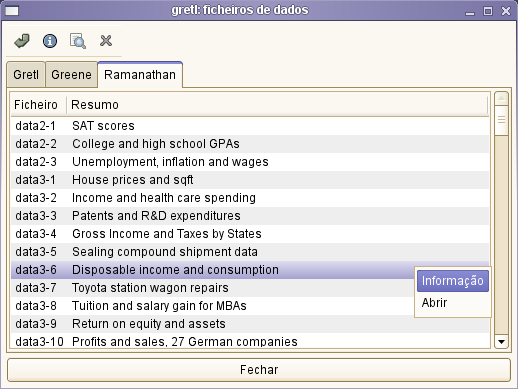
\includegraphics{datafiles}
    \caption{Practice data files window}
    \label{fig:dfiles}
  \end{center}
\end{figure}

If you select a row in this window and click on ``Info'' this pops
open the the ``header file'' for the data set in question, which tells
you something about the source and definition of the variables.  If
you find a file that is of interest, you may open it by clicking on
``Open'', or just double-clicking on the file name.  For the moment
let's open \texttt{data3-6}.

\tip{In \textsc{gretl} windows containing lists, double-clicking on a
  line launches a default action for the associated list entry:
  e.g.\ displaying the values of a data series, opening a file.}

This file contains data pertaining to a classic econometric
``chestnut'', the consumption function.  The data window should now
display the name of the current data file, the overall data range and
sample range, and the names of the variables along with brief
descriptive tags---see Figure~\ref{fig:mainwin}.

\begin{figure}[htbp]
  \begin{center}
    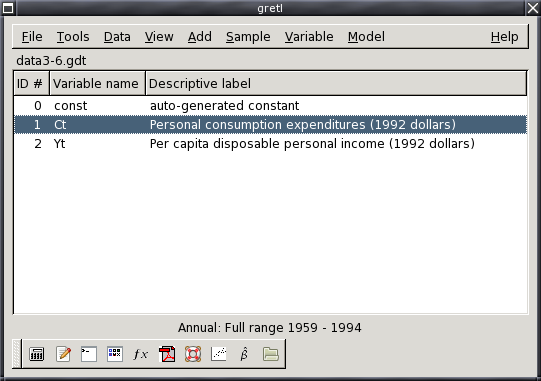
\includegraphics{mainwin}
    \caption{Main window, with a practice data file open}
    \label{fig:mainwin}
  \end{center}
\end{figure}

OK, what can we do now?  Hopefully the various menu options should be
fairly self explanatory.  For now we'll dip into the Model menu; a
brief tour of all the main window menus is given in
section~\ref{menus} below.

\textsc{gretl}'s Model menu offers numerous various econometric
estimation routines.  The simplest and most standard is Ordinary Least
Squares (OLS).
  
Selecting OLS pops up a dialog box calling for a \textit{model
  specification}.  This takes the form of a list of variable names or
numbers, separated by spaces.  The first name or number represents the
dependent variable, the remainder the independent variables.  It is
usual to include a constant (ID number 0) among the independent
variables (otherwise you are forcing the intercept to equal zero).

  \tip{You can put a variable's ID number into the dialog box by
    clicking on that variable's row in the main window.}

Thus, continuing the example of \texttt{data3-6}, the entry
\begin{center}
  \texttt{2 0 3} (or equivalently \texttt{Ct 0 Yt})
\end{center}
specifies a regression of consumption (dependent) on income and a
constant.

You can specify a lagged value of an existing variable without
explicitly adding this to the data set first.  Thus a variant on the
above estimation command which includes the first lag of income on the
right-hand side would be
\begin{center}
  \texttt{2 0 3 Yt(-1)}
\end{center}
The lag is selected using a negative integer enclosed in parentheses.
Note that in this context the name, not the number, of the variable in
question must be used.

\section{Estimation output}
\label{estout}

Once you've specified a model, a window displaying the regression
output will appear.  The output is reasonably comprehensive and in a
standard format.  

The output window contains menus that allow you to inspect or graph
the residuals and fitted values, and to run various diagnostic tests
on the model.  

There is also an option to reprint the regression output in \LaTeX{}
format.  This is not fully implemented yet, but works for OLS
models.  You can print the results in a tabular format (similar to
what's in the output window, but properly typeset) or as an equation,
across the page.  For each of these options you can choose to preview
the typeset product, or save the output to file for incorporation in a
\LaTeX{} document.  Previewing requires that you have a functioning
\TeX{} system on your computer.

If you want to import \textsf{gretl} output into an editor or word
processor there are two main options.  You can simply copy and paste
from an output window (using its Edit menu) to the target program, or
you can save the output to a file then import the file into the target
program.  When you finish a \textsf{gretl} session you are given the
option of saving all the output from the session to a single file.

\tip{When inserting \textsc{gretl} output into a word processor,
  select a monospaced or typewriter-style font (e.g.\ Courier) to
  preserve the output's tabular formatting.  Select a small font
  (10-point Courier should do) to prevent the output lines from being
  broken in the wrong place.}

\section{The main window menus}
\label{menus}

Reading left to right along the main window's menu bar, we find 
the File, Session, Data, Sample, Variable, Model and Help menus (see
Figure~\ref{fig:mainwin}).  

\begin{itemize}
\item \textsf{File menu} 
  \begin{itemize}
  \item \textit{Open data}: Open a native \textsc{gretl} data file or
    import from other formats.  See section~\ref{dfiles}.
  \item \textit{Clear data set}: Clear the current data set out of
    memory.  Generally you don't have to do this (since opening a new
    data file automatically clears the old one) but sometimes it's
    useful (see section ~\ref{scratch}).
  \item \textit{Browse databases}: See sections~\ref{dbase} and
    \ref{scratch}.
  \item \textit{Save data} and \textit{Export data}: Write out the
    current data set in native format, in Comma Separated Values (CSV)
    format, or the formats of GNU R or GNU Octave.  See
    section~\ref{dfiles} and also Appendix C.
  \item \textit{Create data set}: Initialize the built-in spreadsheet
    for entering data manually.  See section~\ref{scratch}.
  \item \textit{Save last graph}: Just as it says.
  \item \textit{Open command file}: Open a file of \textsc{gretl}
    commands, either one you have created yourself or one of the
    practice files supplied with the package.  If you want to create a
    command file from scratch use the next item, \textit{New command
      file}.
  \item \textit{Gretl console}: Open a ``console'' window into which
    you can type commands as you would using the command-line program,
    \textsf{gretlcli} (as opposed to using point-and-click). See
    section~\ref{cmdref}. 
  \item \textit{p-value finder}: Open a window which enables you to
    look up p-values from the Gaussian, $t$, $\chi^2$, $F$ or gamma
    distributions.  See also the \texttt{pvalue} command in
    section~\ref{cmdref} below. 
  \item \textit{statistical tables}: Look up critical values for
    commonly used distributions (Gaussian, $t$, $\chi^2$, $F$ and
    Durbin--Watson).  
  \item \textit{test calculator}: Calculate test statistics and
    p-values for a range of common hypothesis tests (population mean,
    variance and proportion; difference of means, variances and
    proportions).  The relevant sample statistics must be already
    available for entry into the dialog box.  For some simple tests
    that take as input data series rather than pre-computed sample
    statistics, see ``Difference of means'' and ``Difference of
    variances'' under the Data menu.
  \item \textit{Preferences}: Set the paths to various files
    \textsc{gretl} needs to access.  Choose the font in which gretl
    displays text output.  Select or unselect ``expert mode''. (If
    this mode is selected various warning messages are suppressed.)
    Activate or suppress \textsc{gretl}'s messaging about the
    availability of program updates.  Configure or turn on/off the
    main-window toolbar.
  \item \textit{Exit}: Quit the program.  If expert mode is not
    selected you'll be prompted to save any unsaved work.
  \end{itemize}
  
\item \textsf{Session menu} This is discussed separately below.
  Please see section~\ref{session}.

\item \textsf{Data menu} 
  \begin{itemize}
  \item \textit{Display values}: pops up a window with a simple (not
    editable) printout of the values of the variables (either all of
    them or a selected subset).
  \item \textit{Edit values}: pops up a spreadsheet window where you
    can make changes, add new variables, and extend the number of
    observations.  (The data matrix must remain rectangular, with the
    same number of observations for each series.)
  \item \textit{Graph specified vars}: Gives a choice between a time
    series plot, a regular X--Y scatter plot, an X--Y plot using
    impulses (vertical bars), and an X--Y plot ``with factor
    separation'' (i.e.\ with the points colored differently depending
    to the value of a given dummy variable).  Serves up a dialog box
    where you specify the variables to graph.  The simplest way to
    fill out the dialog entry is to refer to the variables by their ID
    numbers (shown in the leftmost column of the main data window).
    Thus, having chosen the scatter plot option, an entry of ``2 3''
    will plot variable number 2 (here, consumption) against variable
    number 3 (income).  The last referenced variable will be on the
    $x$ axis.  Gnuplot is used to render the graph.
  \item \textit{Multiple scatterplots}: Show a collection of (at most
    six) pairwise plots, with either a given variable on the $y$ axis
    plotted against several different variables on the $x$ axis, or
    several $y$ variables plotted against a given $x$.  May be useful
    for exploratory data analysis.
  \item \textit{Read info}, \textit{Edit header}: ``Read info'' just
    displays the header file information for the current data file;
    ``Edit header'' allows you to make changes to it (if you have
    permission to do so).
  \item \textit{Summary statistics}: shows a fairly full set of
    descriptive statistics for all variables in the data set.
  \item \textit{Correlation matrix}: shows the pairwise correlation
    coefficients for the variables in the data set.
  \item \textit{Difference of means}: calculates the $t$ statistic for
    the null hypothesis that the population means are equal for two
    selected variables and shows its p-value.
  \item \textit{Difference of variances}: calculates the $F$ statistic
    for the null hypothesis that the population variances are equal for
    two selected variables and shows its p-value.
  \item \textit{Add variables}: gives a sub-menu of standard
    transformations of variables (logs, lags, squares, etc.) that you
    may wish to add to the data set.  Also gives the option of adding
    random variables, and (for time-series data) adding seasonal dummy
    variables (e.g.\ quarterly dummy variables for quarterly data).
    Includes an item for seeding the program's pseudo-random number
    generator.  
  \item \textit{Refresh window}: Sometimes \textsf{gretl} commands
    generate new variables.  The ``refresh'' item ensures that the
    listing of variables visible in the main data window is in sync
    with the program's internal state.
  \end{itemize}

\item \textsf{Sample menu}
  \begin{itemize}
  \item \textit{Set range}: Select a different starting and/or
    ending point for the current sample, within the range of data
    available. 
  \item \textit{Restore full range}: self-explanatory.
  \item \textit{Set frequency, startobs}: Impose a particular
    interpretation of the data in terms of frequency and starting
    point.  This is primarily intended for use with panel data; see
    section~\ref{panel} below.  
  \item \textit{Define, based on dummy}: Given a dummy (indicator)
    variable with values 0 or 1, this drops from the current sample
    all observations for which the dummy variable has value 0.
  \item \textit{Restrict, based on criterion}: Similar to the item
    above, except that you don't need a pre-defined variable: you
    supply a Boolean expression (e.g.\ \texttt{sqft > 1400}) and the
    sample is restricted to observations satisfying that condition.
    See the help for \texttt{genr} in section~\ref{cmdref} for details
    on the Boolean operators that can be used.
  \item \textit{Drop all obs with missing values}: Drop from the
    current sample all observations for which at least one variable
    has a missing value (see section~\ref{missing} below).
  \item \textit{Count missing values}: Give a report on observations
    where data values are missing.  May be useful in examining a panel
    data set, where it's quite common to encounter missing values.
  \item \textit{Add case markers}: Prompts for the name of a text file
    containing ``case markers'' (short strings identifying the
    individual observations) and adds this information to the data
    set.  See section~\ref{dfiles} below.
  \end{itemize}

\item \textsf{Variable menu} Most items under here operate on a single
  variable at a time.  The ``active'' variable is set by highlighting
  it (clicking on its row) in the main data window.  Most options
  will be self-explanatory.  Note that you can rename a variable,
  and can edit its descriptive label.  
  
  You can also ``Define a new variable'' via a formula (e.g.\ 
  involving some function of one or more existing variables).  For the
  syntax of such formulae, look at the online help for ``Generate
  variable syntax'' or see the \texttt{genr} command in
  section~\ref{cmdref} below.  One simple example:
\begin{center}
\texttt{foo = x1 * x2} 
\end{center}
will create a new variable \texttt{foo} as the product of the existing
variables \texttt{x1} and \texttt{x2}.  In these formulae, variables
must be referenced by name, not number. 

\item \textsf{Model menu} This is introduced in section~\ref{start}.
  For details on the various estimators offered under this menu please
  consult sections~\ref{estim} and ~\ref{cmdref} below, and/or the
  online help under ``Help, Estimation''.

\item \textsf{Help menu}  Please use this as needed!  It gives details
  on the syntax required in various dialog entries.   

\end{itemize}

\section{Command scripts}
\label{scripts}

As you execute commands in \textsf{gretl}, using the GUI and filling
in dialog entries, those commands are recorded in the form of a
``script''.  Such scripts can be edited and re-run, using
either \textsf{gretl} or the command-line client, \textsf{gretlcli}.

To view the current state of the script at any point in a
\textsf{gretl} session, choose ``Command log'' under the File menu.
This log is called \texttt{session.inp} and it is overwritten whenever
you start a new session.  To preserve it, save the script under a
different name.  Script files will be found most easily, using the GUI
file selector, if you name them with the extension ``\texttt{.inp}''.

To open a script you have written independently, use the ``File, Open
command file'' menu item.

With a script window open, use its ``File, Save and Run'' menu item to
run the commands.  All output is directed to a single window, where it
can be edited, saved or copied to the clipboard.

To learn more about the possibilities of scripting, take a look at the
\textsf{gretl} Help item ``Script commands syntax,'' or start up the
command-line program \textsf{gretlcli} and consult its help, or
consult section~\ref{cmdref} of this manual.  In addition, the
\textsf{gretl} package includes over 70 ``practice'' scripts.  Most of
these relate to Ramanathan (1998), but they may also be used as a
free-standing introduction to scripting in \textsf{gretl} and to
various points of econometric theory.  You can explore the practice
files under ``File, Open command file, practice file''  There you
will find a listing of the files along with a brief description of the
points they illustrate and the data they employ.  Open any file and
run it (``File, Run'' in the resulting script window) to see the
output.

Note that long commands in a script can be broken over two or more
lines, using backslash as a continuation character.

You can, if you wish, use the GUI controls and the scripting
approach in tandem, exploiting each method where it offers greater
convenience.  Here are two suggestions.

\begin{itemize}
\item Open a data file in the GUI.  Explore the data---generate
  graphs, run regressions, perform tests.  Then open the Command log,
  edit out any redundant commands, and save it under a specific name.
  Run the script to generate a single file containing a concise record
  of your work.
\item Start by establishing a new script file.  Type in any commands
  that may be required to set up transformations of the data (see the
  \texttt{genr} command in section~\ref{cmdref} below).  Typically
  this sort of thing can be accomplished more efficiently via commands
  assembled with forethought rather than point-and-click.  Then save
  and run the script: the GUI data window will be updated accordingly.
  Now you can carry out further exploration of the data via the GUI.
  To revisit the data at a later point, open and rerun the
  ``preparatory'' script first.
\end{itemize}

A further option is available for your computing convenience.  Under
\textsf{gretl}'s File menu you will find the item ``Gretl console''.
This opens up a window in which you can type commands and execute them
one by one (by pressing the Enter key) interactively.  This is
essentially the same as \textsf{gretlcli}'s mode of operation, except
that (a) the GUI is updated based on commands executed from the
console, enabling you to work back and forth as you wish, and (b)
\textsc{gretl}'s Monte Carlo loop routine (see section~\ref{monte}) is
not at present available in this mode.

\section{The ``session'' concept}
\label{session}

\textsf{gretl} offers the idea of a ``session'' as a way of keeping
track of your work and revisiting it later.  This is experimental (and
at present more likely to be buggy than the rest of the program): I
would be interested in hearing people's reactions.

The basic idea is to provide a little iconic space containing various
objects pertaining to your current working session (see
Figure~\ref{fig:session}).  You can add objects (represented by icons)
to this space as you go along.  If you save the session, these added
objects should be available again if you re-open the session later.

\begin{figure}[htbp]
  \begin{center}
    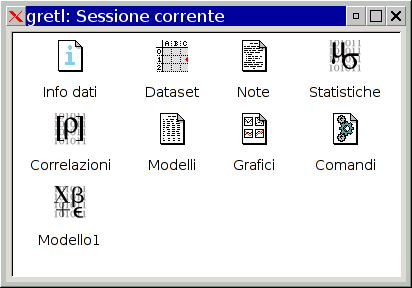
\includegraphics{session}
    \caption{Icon view: one model and one graph have been added to the
      default icons}
    \label{fig:session}
  \end{center}
\end{figure} 

If you start \textsf{gretl} and open a data set, then select ``Icon
view'' from the Session menu, you should see the basic default set of
icons: these give you quick access to the command script, information
on the data set (if any), correlation matrix and descriptive summary
statistics.  All of these are activated by double-clicking the
relevant icon.  The ``Data set'' icon is a little more complex:
double-clicking opens up the data in the built-in spreadsheet, but you
can also right-click on the icon for a menu of other actions.  

\tip{In many \textsc{gretl} windows, the right mouse button brings up
  a menu with common tasks.}

Two sorts of objects can be added to the Icon View window: models and
graphs.  

To add a model, first estimate it using the Model menu.  Then pull
down the File menu in the model window and select ``Save to session as
icon...'' or ``Save as icon and close'' (the first of these prompts
you for a name for the model, while the second uses a default name,
e.g.\ ``Model 1'').

To add a graph, first create it (under the Data menu, ``Graph
specified vars'', or via one of \textsf{gretl}'s other
graph-generating commands), then choose ``Add last graph'' from the
Session menu.

Once a model or graph is added its icon should appear in the Icon
View window.  Double-clicking on the icon redisplays the object,
while right-clicking brings up a menu which lets you rename or delete
the object.  This popup menu also gives you the option of editing graphs.

If you create models or graphs that you think you may wish to
re-examine later, then before quitting \textsf{gretl} select ``Save
as...''  from the Session menu and give a name under which to save the
session.  To re-open the session later, either

\begin{itemize}
\item Start \textsf{gretl} then re-open the session file by going to
  the ``Open'' item under the Session menu, or
\item From the command line, type \texttt{gretl -r}
  \textit{sessionfile}, where \textit{sessionfile} is the name under
  which the session was saved.
\end{itemize}

Also under the Session menu is an option to launch a GNU R session.  R
is a separate program (see Appendix C): if R is not installed on your
computer this menu item will not accomplish anything.  This is a
convenience function for anyone wishing to carry out further
statistical analyses not available in \textsc{gretl}: when R is
invoked in this way, it comes up loaded with a copy of the current
\textsc{gretl} data set.

\section{The gretl toolbar}
\label{toolbar}

At the bottom left of the main window sits the toolbar.  The icons
have the following functions, reading from left to right:  

\begin{enumerate}
\item Launch a calculator program.  This is just a convenience
  function in case you want quick access to a calculator when you're
  working in \textsf{gretl}.  The default program is \texttt{calc.exe}
  under MS Windows, or \texttt{xcalc} under the X window system.  You
  can change the program under the ``File, Preferences, General''
  menu, ``Toolbar'' tab.
\item Launch an editor or word processor.  The default is
  \texttt{winword.exe} under MS Windows, \texttt{emacs} under X.  This
  is configurable in the same way as the calculator launcher.
\item Open the gretl console.  A shortcut to the ``Gretl console''
  menu item (section~\ref{menus} above).
\item Open the \textsc{gretl} website in your web browser.  This will
  work only if you are connected to the Internet and have a properly
  configured browser.
\item Open the current version of this manual, in PDF format.  As with
  the previous item, this requires an Internet connection; it also
  requires that your browser knows how to handle PDF files.
\item A shortcut to the help item for script commands syntax (i.e. a
  listing with details of all available commands).
\item Shortcut to dialog box for defining a graph.
\item Shortcut to the listing of datasets associated with Ramanathan's
  \textit{Introductory Econometrics}.
\end{enumerate}

If you don't care to have the toolbar displayed, you can turn it off
under the ``File, Preferences, General'' menu.  Go to the Toolbar tab
and uncheck the ``show gretl toolbar'' box.


\section{Data files}
\label{dfiles}

\subsection{Basic native format}

In \textsc{gretl}'s native data format, a data set is represented by
two files.  One contains the actual data and the other information on
how the data should be read.  To be more specific:

\begin{enumerate}
  
\item \textit{Actual data}: A rectangular matrix of white-space
  separated numbers.  Each column represents a variable, each row an
  observation on each of the variables (spreadsheet style). Data
  columns can be separated by spaces or tabs. The filename should have
  either no suffix or the suffix \texttt{.dat}.  By default the data
  file is ASCII (plain text).  Optionally it can be gzip-compressed to
  save disk space.
  
  You can insert comments into a data file: if a line begins with the
  hash mark (\texttt{\#}) the entire line is ignored.  This is
  consistent with gnuplot and octave data files.
  
\item \textit{Header}: The data file must be accompanied by a
  header file which has the same basename as the
  data file plus the suffix \texttt{.hdr}.  This file contains, in
  order:

  \begin{itemize}
  \item (Optional) \textit{comments} on the data, set off by the
    opening string \texttt{(*} and the closing string \texttt{*)},
    each of these strings to occur on lines by themselves.
  \item (Required) list of white-space separated \textit{names of the
      variables} in the data file.  Names are limited to 8 characters,
    must start with a letter, and are limited to alphanumeric
    characters plus the underscore.  The list may continue over more
    than one line; it is terminated with a semicolon, \texttt{;}.
  \item (Required) \textit{observations} line of the form \texttt{1 1
      85}.  The first element gives the data frequency (1 for undated
    or annual data, 4 for quarterly, 12 for monthly).  The second and
    third elements give the starting and ending observations.
    Generally these will be 1 and the number of observations
    respectively, for undated data.  For time-series data one can use
    dates of the form \texttt{1959.1} (quarterly, one digit after the
    point) or \texttt{1967.03} (monthly, two digits after the point).
    See section~\ref{panel} below for special use of this line in the
    case of panel data.
  \item The keyword \texttt{BYOBS}. 
  \end{itemize}
\end{enumerate}

Here is an example of a well-formed data header file.

\begin{verbatim}
(*
DATA9-6:
  Data on log(money), log(income) and interest rate from US.
  Source: Stock and Watson (1993) Econometrica (unsmoothed data)
  Period is 1900-1989 (annual data).  
  Data compiled by Graham Elliott.
*)
lmoney lincome intrate ;
1 1900 1989
BYOBS
\end{verbatim}

The corresponding data file contains three columns of data, each
having 90 entries.

\subsection{Extensions to the basic data format}

The options available in \textsc{gretl} data files are broader than
the setup just described, in three ways:

\begin{enumerate}
\item If the \texttt{BYOBS} keyword is replaced by \texttt{BYVAR}, and
  followed by the keyword \texttt{BINARY}, this indicates that the
  corresponding data file is in binary format.  Such data files can be
  written from \textsf{gretlcli} using the \texttt{store} command with
  the \texttt{-s} flag (single precision) or the \texttt{-o} flag
  (double precision). 
\item If \texttt{BYOBS} is followed by the keyword \texttt{MARKERS},
  \textsc{gretl} expects a data file in which the \textit{first
    column} contains strings (8 characters maximum) used to identify
  the observations.  This may be handy in the case of cross-sectional
  data where the units of observation are identifiable: countries,
  states, cities or whatever.  It can also be useful for irregular
  time series data, such as daily stock price data where some days are
  not trading days---in this case the observations can be marked with
  a date string such as \texttt{10/01/98}.  (Remember the 8-character
  maximum.)  Note that \texttt{BINARY} and \texttt{MARKERS} are
  mutually exclusive flags.  Also note that the ``markers'' are not
  considered to be a variable: this column does not have a
  corresponding entry in the list of variable names in the header
  file.
\item If a file with the same base name as the data file and header
  files, but with the suffix \texttt{.lbl}, is found, this is read to
  fill out the descriptive labels for the data series.  The format of
  the (plain text) label file is simple: each line contains the name
  of one variable (as found in the header file), followed by one or
  more spaces, followed by the descriptive label.  Here is an example:

\begin{verbatim}
price  New car price index, 1982 base year
\end{verbatim}
  
  A label file of this sort is created automatically when you save
  data from \textsf{gretl}, if there is any descriptive information to
  be saved.  Such information can be added under the ``Variable, Edit
  label'' menu item.

\end{enumerate}

\subsection{Other data file formats}
\label{csvetc}

\textsc{gretl} will read various other data formats.

\begin{itemize}
  
\item Comma-Separated Values (CSV) files.  These can be brought in
  using \textsf{gretl}'s ``File, Open Data, Import CSV...'' menu item,
  or the \texttt{import} script command.  The program expects a file
  that has (a) valid variable names on the first row and (b) a
  rectangular block of data beneath.  Optionally the first column may
  contain strings such as dates (8 characters max.): such a column
  should be headed ``\texttt{obs}'' or ``\texttt{date}'', or its first
  row cell may be left blank.  There should be \textit{exactly one}
  non-data row at the top of the file.  See also section~\ref{scratch}
  below.
  
\item BOX1 format data.  Large amounts of micro data are available
  (for free) in this format via the Data Extraction Service of the US
  Bureau of the Census.  See
 
  \url{http://www.census.gov/ftp/pub/DES/www/welcome.html}
  
  BOX1 data may be imported using the ``File, Open Data, Import
  BOX...'' menu item or the \texttt{import -o} script command.

\end{itemize}

When you import data from either of these two formats, \textsf{gretl}
opens a ``diagnostic'' window, reporting on its progress in reading
the data.  If you encounter a problem with ill-formatted data, the
messages in this window should give you a handle on fixing the
problem.

For the convenience of anyone wanting to carry out more complex data
analysis, \textsc{gretl} has a facility for writing out data in the
native formats of GNU R and GNU Octave (see Appendix C).  In the GUI
client this option is found under the ``File'' menu; in the
command-line client use the \texttt{store} command with the flag
\texttt{-r} (R) or \texttt{-m} (Octave).

\section{Binary databases}
\label{dbase}
  
For working with large amounts of data I have supplied \textsf{gretl}
with a database-handling routine.  A \textit{database}, as opposed to
a \textit{data file}, is not read directly into the program's
workspace.  A database can contain series of mixed frequencies and
sample ranges.  You open the database and select series to import
into the working data set.  You can then save those series in a native
format data file if you wish.  Databases can be accessed via
\textsf{gretl}'s menu item ``File, Browse databases''.
  
A \textsc{gretl} database consists of two parts: an ASCII index file
(with filename suffix \texttt{.idx}) containing information on the
series, and a binary file (suffix \texttt{.bin}) containing the actual
data.  Two examples of the format for an entry in the \texttt{idx}
file are shown below:

\begin{verbatim}
G0M910    Composite index of 11 leading indicators (1987=100)
M 1948.01 - 1995.11  n = 575
\end{verbatim}

\begin{verbatim}
currbal Balance of Payments: Balance on Current Account; SA
Q 1960.1 - 1999.4 n = 160
\end{verbatim}
  
The first field is the series name.  The second is a description of
the series (maximum 128 characters).  On the second line the first
field is a frequency code: \texttt{M} for monthly, \texttt{Q} for
quarterly and \texttt{A} for annual.  No other frequencies are
accepted at present.  Then comes the starting date (N.B. with two
digits following the point for monthly data, one for quarterly data,
none for annual), a space, a hyphen, another space, the ending date,
the string `` \texttt{n = }'' and the integer number of observations.
This format must be respected exactly.

Optionally, the first line of the index file may contain a short
comment (64 characters) on the source and nature of the data,
following a hash mark.  For example:

\begin{verbatim}
# Federal Reserve Board (interest rates)
\end{verbatim}

The corresponding binary database file holds the data values,
represented as ``floats'', that is, single-precision floating-point
numbers, typically taking four bytes apiece.  The numbers are packed
``by variable'', so that the first $n$ numbers are the observations of
variable 1, the next $m$ the observations on variable 2, and so on.

\subsection{Online access to databases}

As of version 0.40, \textsf{gretl} is able to access databases via the
internet.  Several databases are available from Wake Forest
University.  Your computer must be connected to the internet for this
option to work.  Please see the item on ``Online databases'' under
\textsf{gretl}'s Help menu.  Expect to see this facility developed
further in future releases.

\subsection{RATS 4 databases}

Thanks to Thomas Doan of \textit{Estima}, who provided me with the
specification of the database format used by RATS 4 (Regression
Analysis of Time Series), \textsf{gretl} can also handle such
databases.  Well, actually, a subset of same: I have only worked on
time-series databases containing monthly and quarterly series.  My
university has the RATS G7 database containing data for the seven
largest OECD economies and \textsf{gretl} will read that OK.

\tip{Visit the \textsc{gretl} data page at
  \url{http://ricardo.ecn.wfu.edu/gretl/gretl_data.html} for details
  and updates on available data.}
 
\section{Missing data values}
\label{missing}

These are represented internally as $-999$.  In a native-format data
file they should be represented the same way.  When importing CSV data
\textsc{gretl} accepts any of three representations of missing values:
$-999$, the string \texttt{NA}, or simply a blank cell.  Blank cells
should, of course, be properly delimited, e.g.\ \texttt{120.6,,5.38},
in which the middle value is presumed missing.

As for handling of missing values in the course of statistical
analysis, \textsc{gretl} does the following:

\begin{itemize}
\item In calculating descriptive statistics (mean, standard deviation,
  etc.) under the \texttt{summary} command, missing values are simply
  skipped and the sample size adjusted appropriately.
\item In running regressions \textsc{gretl} first adjusts the
  beginning and end of the sample range, truncating the sample if need
  be.  Missing values at the beginning of the sample are common in
  time series work due to the inclusion of lags, first differences and
  so on; missing values at the end of the range are not uncommon due
  to differential updating of series and possibly the inclusion of
  leads.  
\item If \textsc{gretl} detects any missing values ``inside'' the
  (possibly truncated) sample range for a regression it gives an error
  message and refuses to produce estimates.
\end{itemize}

Missing values in the middle of a data set are a problem.  In a
cross-sectional data set it may be possible to move the offending
observations to the beginning or the end of the file, but obviously
this won't do with time series data.  For those who know what they are
doing (!), the \texttt{misszero} function is provided under the
\texttt{genr} command.  By doing 

\begin{verbatim}
genr foo = misszero(bar)
\end{verbatim}

you can produce a series \texttt{foo} which is identical to
\texttt{bar} except that any $-999$ values become zeros.  Then you can
use carefully constructed dummy variables to, in effect, drop the
missing observations from the regression while retaining the
surrounding sample range.\footnote{\texttt{genr} also offers the inverse
function to \texttt{misszero}, namely \texttt{zeromiss}, which replaces
zeros in a given series with the missing observation code.}

\section{Creating a data file from scratch}
\label{scratch}

There are four ways to do this: (1) Use your favorite text editor to
create the data file and header file independently.
(2) Use your favorite spreadsheet to establish the data file, save it
in Comma Separated Values format, then use \textsf{gretl}'s ``Import
CSV'' option. (3) Use \textsf{gretl}'s built-in spreadsheet. (4)
Select data series from a suitable database.

Here are a few comments and details on these methods.

\begin{enumerate}
\item \textit{Using a text editor}.  This may be the method of choice
  for those who have a strong preference in editors, and who don't
  mind taking a few minutes to study the specifications for valid data
  and header files, as set out in section~\ref{dfiles} above.

  Note that this method can be problematic under MS Windows due to
  the propensity of Microsoft tools ``helpfully'' to add the suffix
  \texttt{.txt} to the filename you specify when you save a plain text
  file---even if it already has a suffix.  This will render the files
  unusable with \textsf{gretl}: you'll have to rename them
  manually, outside of the editor.
  
\item \textit{Using a separate spreadsheet}.  This may be a good
  choice if you're comfortable with a particular spreadsheet.  Of
  course if you use a spreadsheet you're able to carry out various
  transformations of the ``raw'' data with ease (adding things up,
  taking percentages or whatever): note, however, that you can also do
  this sort of thing easily---perhaps more easily---within
  \textsf{gretl}, by using the tools under the ``Data, Add variables''
  menu and/or ``Variable, define new variable''.

  If you take this option, please pay attention to the specification
  of what your spreadsheet should look like before you save it in CSV
  format (section~\ref{csvetc}).
  
  You may wish to establish a \textsc{gretl} data set piece by piece,
  via incremental importation of CSV data.  This is supported as
  follows.  When you have a datafile open already, and then select the
  menu item ``File, Open data, import CSV...'' the program checks for
  conformability between the existing data set and the new import.  If
  the data frequency, starting observation and ending observation all
  seem to match, the new data are merged into the data set.  If not,
  an error message is printed and the import is refused.  If you want
  to import the new data \textit{in place of} the existing data set,
  you can achieve this by first selecting ``File, Clear data set''.
  
\item \textit{Built-in spreadsheet}.  Under \textsf{gretl}'s ``File,
  Create data set'' menu you can choose the sort of data set you want
  to establish (e.g.\ quarterly time series, cross-sectional).  You
  will then be prompted for starting and ending dates (or observation
  numbers) and the name of the first variable to add to the data set.
  After supplying this information you will be faced with a simple
  spreadsheet into which you can type data values.  In the spreadsheet
  window, clicking the right mouse button will invoke a popup menu
  which enables you to add a new variable (column), to add an
  observation (append a row at the foot of the sheet), or to insert an
  observation at the selected point (move the data down and insert a
  blank row.)
  
  Once you have entered data into the spreadsheet you import these
  into \textsf{gretl}'s workspace using the spreadsheet's ``File,
  Apply changes'' menu item.

  Please note that \textsf{gretl}'s spreadsheet is quite basic and
  has no support for functions or formulas.  Data transformations are
  done via the ``Data'' or ``Variable'' menus in the main
  \textsf{gretl} window.  

\item \textit{Selecting from a database}.  The remaining alternative
  is to establish your data set by selecting variables from a
  database.  \textsc{gretl} comes with a database of US macroeconomic
  time series and, as mentioned above, the program will reads RATS 4
  databases.  
  
  Begin with \textsf{gretl}'s ``File, Browse databases'' menu item.
  This has three forks: ``gretl native'', ``RATS 4'' and ``on database
  server''.  You should be able to find the file \texttt{bcih.bin} in
  the file selector that opens if you choose the ``gretl native''
  option---this file is supplied with the distribution.
  
  You won't find anything under ``RATS 4'' unless you have purchased
  RATS data (see \url{www.estima.com}).  If you do possess RATS data
  you should go into \textsf{gretl}'s ``File, Preferences, General''
  dialog, select the Databases tab, and fill in the correct path to
  your RATS files.
  
  If your computer is connected to the internet you should find
  several databases (at Wake Forest University) under ``on database
  server''.  You can browse these remotely; you also have the option
  of installing them onto your own computer.  The initial remote
  databases window has an item showing, for each file, whether it is
  already installed locally (and if so, if the local version is up to
  date with the version at Wake Forest).

  Assuming you have managed to open a database you can import
  selected series into \textsf{gretl}'s workspace by using the
  ``Import'' menu item in the database window.  
  
  \textit{Note}: \textsf{gretl} has no problem compacting data series
  of relatively high frequency (e.g.\ monthly) to a lower frequency
  (e.g.\ quarterly): this is done by averaging.  But it has no way of
  converting lower frequency data to higher.  Therefore if you want to
  import series of various different frequencies from a database into
  \textsf{gretl} \textit{you must start by importing a series of the
    lowest frequency you intend to use.} This will initialize your
  \textsf{gretl} data set to the low frequency, and higher frequency
  data can be imported subsequently (they will be compacted
  automatically).  If you start with a high frequency series you will
  not be able to import any series of lower frequency.

\end{enumerate}

If you establish a data set by any means other than creating a data
file and header file with a text editor (that is,
if you import CSV, use \textsf{gretl}'s spreadsheet, or select from a
database) you would be well advised to save the data in
\textsf{gretl}'s native format before quitting the program.  You can
do this via the ``File, Save data...'' menu item.

\section{Panel data}
\label{panel}

Panel data (pooled cross-section and time-series) require special
care.  Here are some pointers.

Consider a data set composed of observations on each of $n$
cross-sectional units (countries, states, persons or whatever) in each
of $T$ periods.  Let each observation comprise the values of $m$
variables of interest.  The data set then contains $mnT$ values.

The data should be arranged ``by observation'': each row represents an
observation; each column contains the values of a particular variable.
The data matrix then has $nT$ rows and $m$ columns.  That leaves open
the matter of how the rows should be arranged.  There are two
possibilities.\footnote{If you don't intend to make any conceptual or
  statistical distinction between cross-sectional and temporal
  variation in the data you can arrange the rows arbitrarily, but
  this is probably wasteful of information.}

\begin{itemize}
\item Rows grouped by \textit{unit}.  Think of the data matrix as
  composed of $n$ blocks, each having $T$ rows.  The first block of
  $T$ rows contains the observations on cross-sectional unit 1 for each
  of the periods; the next block contains the observations on unit 2
  for all periods; and so on.  In effect, the data matrix is a set of
  time-series data sets, stacked vertically.
\item Rows grouped by \textit{period}.  Think of the data matrix as
  composed of $T$ blocks, each having $n$ rows.  The first $n$ rows
  contain the observations for each of the cross-sectional units in
  period 1; the next block contains the observations for all units in
  period 2; and so on.  The data matrix is a set of cross-sectional
  data sets, stacked vertically.
\end{itemize}

You may use whichever arrangement is more convenient.  The first is
perhaps easier to keep straight.  If you use the second then of course
you must ensure that the cross-sectional units appear in the same
order in each of the period data blocks.

In either case you can use the frequency field in the
\textit{observations} line of the data header file (see
section~\ref{dfiles}) to make life a little easier.

\begin{itemize}
\item \textit{Grouped by unit}: Set the frequency equal to $T$.
  Suppose you have observations on 20 units in each of 5 time periods.
  Then this observations line is appropriate: \texttt{5 1.1 20.5}
  (read: frequency 5, starting with the observation for unit 1, period
  1, and ending with the observation for unit 20, period 5).  Then,
  for instance, you can refer to the observation for unit 2 in period
  5 as \texttt{2.5}, and that for unit 13 in period 1 as
  \texttt{13.1}.
\item \textit{Grouped by period}: Set the frequency equal to $n$.  In
  this case if you have observations on 20 units in each of 5 periods,
  the observations line should be: \texttt{20 1.01 5.20} (read:
  frequency 20, starting with the observation for period 1, unit 01,
  and ending with the observation for period 5, unit 20).  One refers
  to the observation for unit 2, period 5 as \texttt{5.02}.
\end{itemize}

If you decide to construct a panel data set using a spreadsheet
program first, then bring the data into \textsc{gretl} as a CSV
import, the program will (probably) not at first recognize the special
nature of the data.  You can fix this by using the command
\texttt{setobs} (see section~\ref{cmdref}) or the GUI menu item
``Sample, Set frequency, startobs...''.

\subsection{Dummy variables}

In a panel study you may wish to construct dummy variables of one or
both of the following sorts: (a) dummies as unique identifiers for the
cross-sectional units, and (b) dummies as unique identifiers of the
time periods.  The former can be used, for instance, to allow the
intercept of the regression to differ across the units, the latter to
allow the intercept to differ across periods.  (You will not want to
include all of these dummies in a given regression!)

You can use two special functions to create such dummies.  These are
found under the ``Data, Add variables'' menu in the GUI, or under the
\texttt{genr} command in script mode or \textsf{gretlcli}.

\begin{enumerate}
\item ``periodic dummies'' (script command \texttt{genr dummy}).  The
  common use for this command is to create a set of periodic dummy
  variables up to the data frequency in a time-series study (for
  instance a set of quarterly dummies for use in seasonal adjustment).
  But it also works with panel data.  Note that the interpretation of
  the dummies created by this command differs depending on whether the
  data rows are grouped by unit or by period.  If the grouping is by
  \textit{unit} (frequency $T$) the resulting variables are
  \textit{period dummies} and there will be $T$ of them.  For instance
  \texttt{dummy\_2} will have value 1 in each data row corresponding
  to a period 2 observation, 0 otherwise.  If the grouping is by
  \textit{period} (frequency $n$) then $n$ \textit{unit dummies} will
  be generated: \texttt{dummy\_2} will have value 1 in each data row
  associated with cross-sectional unit 2, 0 otherwise.
\item ``panel dummies'' (script command \texttt{genr paneldum}).  This
  creates all the dummies, unit and period, at a stroke.  The default
  presumption is that the data rows are grouped by unit.  The unit
  dummies are named \texttt{du\_1}, \texttt{du\_2} and so on, while
  the period dummies are named \texttt{dt\_1}, \texttt{dt\_2}, etc.
  The \texttt{u} (for unit) and \texttt{t} (for time) in these names
  will be wrong if the data rows are grouped by period: to get them
  right in that setting use \texttt{genr paneldum -o} (script mode
  only).
\end{enumerate}

If a panel data set has the \texttt{YEAR} of the observation entered
as one of the variables you can create a periodic dummy to pick out a
particular year, e.g.\ \texttt{genr dum = (YEAR=1960)}.  You can also
create periodic dummy variables using the modulus operator,
\texttt{\%}.  For instance, to create a dummy with value 1 for the
first observation and every thirtieth observation thereafter, 0
otherwise, do

\begin{verbatim}
   genr index
   genr dum = ((index-1)%30) = 0
\end{verbatim}

\subsection{Using lagged values with panel data}

If the time periods are evenly spaced you may want to use lagged
values of variables in a panel regression.  In this case arranging the
data rows by \textit{unit} (stacked time-series) is definitely
preferable.

Suppose you create a lag of variable \texttt{x1}, using \texttt{genr
  x1\_1 = x1(-1)}.  The values of this variable will be mostly correct,
but at the boundaries of the unit data blocks they will be spurious
and unusable.  E.g.\ the value assigned to \texttt{x1\_1} for
observation \texttt{2.1} is not the first lag of \texttt{x1} at all,
but rather the last observation of \texttt{x1} for unit 1.

If a lag of this sort is to be included in a regression you must
ensure that the first observation from each unit block is dropped.
One way to achieve this is to use Weighted Least Squares
(\texttt{wls}) using an appropriate dummy variable as weight.  This
dummy (call it \texttt{lagdum}) should have value 0 for the
observations to be dropped, 1 otherwise.  In other words, it is
complementary to a dummy variable for period 1.  Thus if you have
already issued the command \texttt{genr dummy} you can now do
\texttt{genr lagdum = 1 - dummy\_1}.  If you have used \texttt{genr
  paneldum} you would now say \texttt{genr lagdum = 1 - dt\_1}.
Either way, you can now do

\begin{center}
  \texttt{wls lagdum y const x1\_1 ...}
\end{center}

\noindent to get a pooled regression using the first lag of
\texttt{x1}, dropping all observations from period 1.

Another option is to use the \texttt{smpl} with the \texttt{-o} flag
and a suitable dummy variable.  Here are illustrative commands,
assuming the unit data blocks each contain 30 observations and we want
to drop the first row of each:

\begin{verbatim}
   (* create index variable *)
   genr index
   (* create dum = 0 for every 30th obs *)
   genr dum = ((index-1)%30) > 0
   (* sample based on this dummy *)
   smpl -o dum
   (* recreate the obs. structure, for 56 units *)
   setobs 29 1.01 56.29
\end{verbatim}

You can now run regressions on the restricted data set without having
to use the \texttt{wls} command.  If you plan to reuse the restricted
data set you may wish to save it using the \texttt{store} command (see
section~\ref{cmdref} below).

\subsection{Illustration: the Penn World Table}

The Penn World Table (homepage \url{http://pwt.econ.upenn.edu/}) is a
rich macroeconomic panel dataset, spanning 152 countries over the
years 1950--1992.  The data are available in \textsc{gretl} format;
please see \url{http://ricardo.ecn.wfu.edu/gretl/gretl_data.html} (this is
a free download, although it is not included in the main
\textsc{gretl} package).  

Script~\ref{script:pwt} below opens \texttt{pwt56\_60\_89.dat}, a
subset of the pwt containing data on 120 countries, 1960--89, for 20
variables, with no missing observations (the full data set, which is
also supplied in the pwt package for \textsc{gretl}, has many missing
observations).  Total growth of real GDP, 1960--89, is calculated for
each country and regressed against the 1960 level of real GDP, to see
if there is evidence for convergence.

\begin{script}[htbp]
\caption{Example of use of Penn World Table}
\label{script:pwt}
\begin{verbatim}
   open pwt56_60_89.dat
   (* for 1989 (last obs), lag 29 gives 1960, the first obs *)
   genr gdp60 = RGDPL(-29)
   (* find total growth of real GDP over 30 years *)
   genr gdpgro = (RGDPL - gdp60)/gdp60
   (* restrict the sample to a 1989 cross-section *)
   smpl -r YEAR=1989
   (* Convergence?  Have countries with a lower base grown faster? *)
   ols gdpgro const gdp60
   (* result: No! Try inverse relationship *)
   genr gdp60inv = 1/gdp60
   ols gdpgro const gdp60inv
   (* No again.  Try dropping Africa? *)
   genr afdum = CCODE = 1
   genr afslope = afdum * gdp60
   ols gdpgro const afdum gdp60 afslope2
\end{verbatim}
\end{script}

\section{Getting more data}
\label{sec:getting-more-data}

Besides the data files included in the \textsc{gretl} distribution and
the Penn World Table mentioned above, a large collection of data of
various sorts is available in a form directly readable by
\textsc{gretl} via the web page
\url{http://www.ecn.wfu.edu/gretl/gretl_data.html}.
You will find details on that page.  Data sources include the Board of
Governors of the Federal Reserve System (U.S. interest rates), the
Federal Reserve Bank of St.\ Louis (numerous U.S. macroeconomic time
series, up to the present), The National Bureau of Economic Research
(their ``macro history'' data collection, plus some international and
industry-level data sets), and the Bank of Japan.

In addition \textsc{gretl} comes with some scripts that can be used to
create databases using data available via the Internet. These can be
found in the \texttt{utils} subdirectory of the source package (see
section~\ref{intro} above). To run the scripts you need to have
\textsf{perl} installed on your computer, and you need to be connected
to the Internet.

\section{Graphs and plots}
\label{graph}

A separate program, namely gnuplot, is called to generate graphs.
Gnuplot is a very full-featured graphing program with myriad options.
It is available from \url{www.gnuplot.org} (but note that a copy of
gnuplot is bundled with the MS Windows version of \textsc{gretl}).
\textsf{gretl} gives you direct access, via a graphical interface, to
only a small subset of gnuplot's options but it tries to choose
sensible values for you; it also allows you to take complete control
over graph details if you wish.

Under MS Windows you can click at the top left corner of a graph
window for a pull-down gnuplot menu that lets you choose various
things (including copying the graph to the Windows clipboard and
sending it to a printer).

For full control over a graph, follow this procedure:

\begin{enumerate}
\item Close the graph window.
\item From the Session menu, choose ``Add last graph''.
\item In the session icon window, right-click on the new graph icon
  and choose either ``Edit using GUI'' or ``Edit plot commands''.
\end{enumerate}

The ``Edit using GUI'' item pops up a graphical controller for gnuplot
which lets you fine-tune various aspects of the graph.  The ``Edit
plot commands'' item opens an editor window containing the actual
gnuplot command file for generating the graph: this gives you full
control over graph details---if you know something about gnuplot. To
find out more, see \url{http://ricardo.ecn.wfu.edu/gnuplot.html} or
\url{www.gnuplot.org}.

% You should be able to get the graph
%   looking pretty much as you wish with the controls provided (see
%   Figure~\ref{fig:plot}).  But again, if you want yet more control,
%   choose the ``plot commands'' output option then open the commands
%   file in gnuplot.  Note to power users: When you open a graph ``with
%   controls'', under the Main tab in the controller box you'll find two
%   pull-down menus, for ``key position'' and ``output type''.  Besides
%   the preconfigured options, you can type custom strings in there.  A
%   custom string typed into ``key position'' will be appended to
%   ``\texttt{set key}'' and passed to gnuplot, while a custom entry
%   under ``output type'' will be appended to ``\texttt{set term}'' and
%   again passed to gnuplot.  Thus you can gain an extra degree of
%   control even without using the option of saving a file of gnuplot
%   commands.

See also the entry for \texttt{gnuplot} in section~\ref{cmdref}
below---and the \texttt{graph} and \texttt{plot} commands for 
``quick and dirty'' ASCII graphs.

\begin{figure}[htbp]
  \begin{center}
    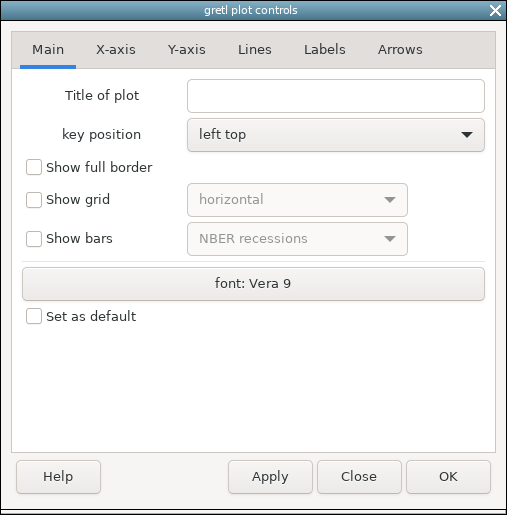
\includegraphics{plot_control}
    \caption{gretl's gnuplot controller}
    \label{fig:plot}
  \end{center}
\end{figure}

\section{Monte Carlo simulations}
\label{monte}

\textsc{gretl} offers (limited) support for Monte Carlo simulations.
To do such work you should either use the GUI client program in
``script mode'' (section~\ref{scripts} above), or use the command-line
client.  The command \texttt{loop} opens a special mode in which the
program accepts commands to be repeated a specified number of times.
Within such a loop, only four commands can be used: \texttt{genr},
\texttt{ols}, \texttt{print} and \texttt{store}.  With \texttt{genr}
and \texttt{ols} it is possible to do quite a lot. You exit the mode
of entering loop commands with \texttt{endloop}: at this point the
stacked commands are executed.  Loops cannot be nested.

The \texttt{ols} command gives special output in a loop context: the
results from each individual regression are not printed, but rather
you get a printout of (a) the mean value of each estimated coefficient
across all the repetitions, (b) the standard deviation of those
coefficient estimates, (c) the mean value of the estimated standard
error for each coefficient, and (d) the standard deviation of the
estimated standard errors.  This makes sense only if there is some
random input at each step.  

The \texttt{print} command also behaves differently in the context of
a loop.  It prints the mean and standard deviation of the variable,
across the repetitions of the loop.  It is intended for use with
variables that have a single value at each iteration, for example the
error sum of squares from a regression.

The \texttt{store} command (use only one of these per loop) writes out
the values of the specified variables, from each time round the loop,
to the specified file.  Thus it keeps a complete record of the
variables.  This data file can then be read into the program and
analysed.

A simple example of loop code is shown in Script~\ref{script:loop}.

\begin{script}[htbp]
\caption{Example Monte Carlo code}
\label{script:loop}
\begin{verbatim}
   (* create a blank data set with series length 50 *)
   nulldata 50
   genr x = uniform()
   (* open a loop, to be repeated 100 times *)
   loop 100
      genr u = normal()
      (* construct the dependent variable *)
      genr y = 10*x + 20*u
      (* run OLS regression *)
      ols y const x
      (* grab the R-squared value from the regression *)
      genr r2 = $rsq
      (* arrange for statistics on R-squared to be printed *)
      print r2
      (* save the individual coefficient estimates *)
      genr a = coeff(const)
      genr b = coeff(x)
      (* and print them to file *)
      store foo.dat a b
   endloop
\end{verbatim}%$
\end{script}

This loop will print out summary statistics for the `a' and `b'
estimates across the 100 repetitions, and also for the $R^2$ values
for the 100 regressions.  After running the loop, \texttt{foo.dat},
which contains the individual coefficient estimates from all the runs,
can be opened in \textsc{gretl} to examine the frequency distribution
of the estimates in detail.  Please note that while comment lines are
permitted in a loop (as shown in the example), they cannot run over
more than one line.

The command \texttt{nulldata} is useful for Monte Carlo work.  Instead
of opening a ``real'' data set, \texttt{nulldata 50} (for instance)
opens an empty data set, with only a constant, with a series length of
50.  Constructed variables can then be added using the \texttt{genr}
command.  

See the \texttt{seed} command in section~\ref{cmdref} for information
on generating repeatable pseudo-random series.

\section{Iterated least squares}
\label{iterate}

A further form of loop structure is provided, designed primarily for
carrying out iterated least squares.  Greene (2000, ch.\ 11) shows how
this method can be used to estimate nonlinear models.

To open this second sort of loop you need to specify a
\textit{condition} rather than an unconditional number of times to
iterate.  This should take the form of the keyword \texttt{while}
followed by an inequality: the left-hand term should be the name of a
variable that is already defined; the right-hand side may be either a
numerical constant or the name of another predefined variable.  For
example, 

\begin{verbatim}
loop while essdiff > .00001
\end{verbatim}

Execution of the commands within the loop (i.e.\ until
\texttt{endloop} is encountered) will continue so long as the
specified condition evaluates as true.

I assume that if you specify a ``number of times'' loop you are
probably doing a Monte Carlo analysis, and hence you're not interested
in the results from each individual iteration but rather the moments
of certain variables over the ensemble of iterations.  On the other
hand, if you specify a ``while'' loop you're probably doing something
like iterated least squares, and so you'd like to see the final
result---as well, perhaps, as the value of some variable(s) (e.g.\ the
error sum of squares from a regression) from each time round the loop.
The behavior of the \texttt{print} and \texttt{ols} commands are
tailored to this assumption.  In a ``while'' loop \texttt{print} behaves
as usual; thus you get a printout of the specified variable(s) from
each iteration.  The \texttt{ols} command prints out the results from
the final estimation.  

Script~\ref{script:greene} uses a ``while'' loop to replicate the
estimation of a nonlinear consumption function, of the form $C =
\alpha + \beta Y^{\gamma} + \epsilon$, as presented in Greene (2000,
Example 11.3).  This script is included in the \textsc{gretl}
distribution under the name \texttt{greene11\_3.inp}; you can find it
in \textsf{gretl} under the menu item ``File, Open command file,
practice file, Greene...''.

\begin{script}[htbp]
\caption{Replicate Example 11.3 in Greene}
\label{script:greene}
\begin{verbatim}
open greene11_3.dat
(* run initial OLS *)
ols C 0 Y
genr essbak = $ess
genr essdiff = 1
genr b0 = coeff(Y)
genr gamma0 = 1
(* form the linearized variables *)
genr C0 = C + gamma0 * b0 * Y^gamma0 * log(Y)
genr x1 = Y^gamma0
genr x2 = b0 * Y^gamma0 * log(Y)
(* iterate OLS till the error sum of squares converges *)
loop while essdiff > .00001
   ols C0 0 x1 x2 -o
   genr b0 = coeff(x1)
   genr gamma0 = coeff(x2)
   genr C0 = C + gamma0 * b0 * Y^gamma0 * log(Y)
   genr x1 = Y^gamma0
   genr x2 = b0 * Y^gamma0 * log(Y)
   genr ess = $ess
   genr essdiff = abs(ess - essbak)/essbak
   genr essbak = ess
endloop 
(* print parameter estimates using their "proper names" *)
genr alpha = coeff(0)
genr beta = coeff(x1)
genr gamma = coeff(x2) 
print alpha beta gamma 
\end{verbatim}
\end{script}

% Need section here on ``for i='' loops
% Also need to change the following to reflect opening of databases,
% automatic attempt to distinguish datafiles and scripts.

\clearpage

{
\setlength{\parindent}{0pt}
\setlength{\parskip}{8pt}

\section{Program options and arguments: gretl}
\label{optarg1}

\texttt{gretl}  \qquad (under MS Windows, \texttt{gretlw32})

--- Opens the program and waits for user input.

\texttt{gretl} \textit{datafile}  

--- Starts the program with the specified datafile in its workspace.
The data file may be in native \textsc{gretl} format, CSV format, or
BOX1 format (see section~\ref{dfiles} above).  The program will try to
detect the format of the file and treat it appropriately.  See also
section~\ref{path} below for path-searching behavior.

\texttt{gretl --help} (or \texttt{gretl -h})

--- Prints a brief summary of usage.

\texttt{gretl --version} (or \texttt{gretl -v})

--- Prints version identification for the program.

\texttt{gretl --run} \textit{scriptfile} (or \texttt{gretl -r}
\textit{scriptfile})

--- Start the program and open a window displaying the specified
script file, ready to run.  See section~\ref{path} below for
path-searching behavior.


Some things in \textsf{gretl} are configurable under the ``File,
Preferences'' menu.  

\begin{itemize}
\item The user's base directory for \textsf{gretl}-related files.
\item The base directory for \textsf{gretl}'s shared files.
\item The command to launch GNU R (see Appendix C).
\item The directory in which to start looking for native
  \textsf{gretl} databases.
\item The directory in which to start looking for RATS 4 databases.
\item The IP number of the \textsc{gretl} database server to access.
\item The calculator and editor programs to launch from the toolbar.
\item The monospaced font to be used in \textsf{gretl} screen output.
\end{itemize}

There are also some check boxes.  Checking the ``expert'' box quells
some warnings that are otherwise issued.  Unchecking ``Tell me about
gretl updates'' stops \textsf{gretl} from attempting to query the
update server at start-up.  Unchecking ``Show gretl toolbar'' turns
the icon toolbar off.

Settings chosen in this way are stored in a file named
\texttt{.gretlrc} in the user's home directory on unix-like systems,
or in a file named \texttt{gretl.rc} in the user's gretl directory
(default \verb+c:\userdata\gretl\user+) under MS Windows.

\section{Program options and arguments: gretlcli}
\label{optarg2}

\texttt{gretlcli}  

--- Opens the program and waits for user input.

\texttt{gretlcli} \textit{datafile}  

--- Starts the program with the specified datafile in its workspace.
The data file may be in native \textsc{gretl} format, CSV format, or
BOX1 format (see section~\ref{dfiles} above).  The program will try to
detect the format of the file and treat it appropriately.  See also
section~\ref{path} below for path-searching behavior.

\texttt{gretlcli --help} (or \texttt{gretlcli -h})

--- Prints a brief summary of usage.

\texttt{gretlcli --version} (or \texttt{gretlcli -v})

--- Prints version identification for the program.

\texttt{gretlcli --run} \textit{scriptfile} (or \texttt{gretlcli -r}
\textit{scriptfile})

--- Execute the commands in \textit{scriptfile} then hand over input
to the command line.  See section~\ref{path} below for
path-searching behavior.  

\texttt{gretlcli --batch} \textit{scriptfile} (or \texttt{gretlcli
  -b} \textit{scriptfile})

--- Execute the commands in \textit{scriptfile} then exit.  When using
this option you will probably want to redirect output to a file.  See
section~\ref{path} for path-searching behavior.

When using the \texttt{--run} and \texttt{--batch} options, the script
file in question must call for a data file to be opened.  This can be
done using the \texttt{open} command within the script.  For backward
compatibility with Ramanathan's original ESL program another mechanism
is offered (ESL doesn't have the \texttt{open} command).  A line of
the form:

\texttt{(* ! myfile.dat *)}

will (a) cause \textsf{gretlcli} to load \texttt{myfile.dat}, but
will (b) be ignored as a comment by the original ESL.  Note the
specification carefully: There is exactly one space between the begin
comment marker, ``\texttt{(*}'', and the ``\texttt{!}''; there is
exactly one space between the ``\texttt{!}'' and the name of the data
file.

One further kludge enables \textsf{gretl} and \textsf{gretlcli} to
get datafile information from the ESL ``practice files'' included with
the \textsc{gretl} package.  A typical practice file begins like this:

\texttt{(* PS4.1, using data file DATA4-1, for reproducing Table 4.2
  *)}

This algorithm is used: if an input line begins with the comment
marker, search it for the string ``\texttt{DATA}'' (upper case).  If
this is found, extract the string from the ``\texttt{D}'' up to the
next space or comma, put it into lower case, and treat it as the name
of a data file to be opened.

}

\section{Path searching}
\label{path}

When the name of a data file or script file is supplied to
\textsf{gretl} or \textsf{gretlcli} on the command line
(sections~\ref{optarg1} and \ref{optarg2}), the file is looked for as
follows:

\begin{enumerate}
\item ``As is''.  That is, in the current working directory or, if a
  full path is specified, at the specified location.
\item In the user's gretl directory.  By default this is a directory
  named \texttt{.gretl} in the user's home account, under unix-like
  systems; under MS Windows it is by default a subdirectory named
  \texttt{user} of the \textsc{gretl} installation, e.g. 
  \verb+c:\userdata\gretl\user+.
\item In any immediate sub-directory of the user's gretl directory.
\item In the case of a data file, search continues with the main
  \textsc{gretl} data directory.  By default this is
  \texttt{/usr/local/share/gretl/data} on unix-like systems, or
  \verb+c:\userdata\gretl\data+ under MS Windows.  In the case of a
  script file, the search proceeds to the system script directory,
  by default \texttt{/usr/local/share/gretl/scripts} or
  \verb+c:\userdata\gretl\scripts+.
\item In the case of data files the search then proceeds to all
  immediate sub-directories of the main data directory.
\end{enumerate}

Thus it is not necessary to specify the full path for a data or script
file unless you wish to override the automatic searching mechanism.
(This also applies within \textsf{gretlcli}, when you supply a filename
as an argument to the \texttt{open} or \texttt{run} commands.)

When a command script contains an instruction to open a data file, the
search order for the data file is as stated above, except that the
directory containing the script is also searched, immediately after
trying to find the data file ``as is''.

\subsection{MS Windows}

Under MS Windows the default behavior of \textsf{gretl} and
\textsf{gretlcli} is controlled by the configuration file
\texttt{libgretl.cfg}.  This is first searched for in the directory
containing the \textsf{gretlcli} executable; if it is not found there
it is looked for in the root directory of the current drive (i.e.\ as
\verb+\libgretl.cfg+).  This file specifies, in order, the system
gretl directory, the user's home gretl directory and the path to the
gnuplot executable.  For example, it might read as follows:

\begin{verbatim}
c:\userdata\gretl
c:\userdata\gretl\user
c:\userdata\gp371w32\wgnupl32.exe
\end{verbatim}

When \textsc{gretl} for win32 is installed, a version of this file,
appropriate to the user's choice of where to install the package, is
written out automatically.  You should not have to bother with this
file unless you should happen to want to move a \textsc{gretl}
installation.  In that case you'll have to edit \texttt{libgretl.cfg}
appropriately, maintaining its plain ASCII character and exact
filename (N.B. no stupid ``\texttt{.txt}'' extension as kindly
supplied by MS Notepad!).

\clearpage

\section{Tables of estimators and tests}
\label{estim}

The following are available under the Model menu in \textsf{gretl}'s
main window.  The corresponding script command is shown in
parentheses.  For details consult the command's entry in
section~\ref{cmdref}.


\begin{center}
{\setlength{\extrarowheight}{6pt}
\begin{tabular}{>{\PBS\raggedright\hspace{0pt}}p{2.5in}%
                >{\PBS\raggedright\hspace{0pt}}p{3in}}

\textit{Estimator} & \textit{Comment} \\ [2pt] \hline

Ordinary Least Squares (\texttt{ols}) &  
   The workhorse estimator \\ 
Weighted Least Squares (\texttt{wls}) & 
   Heteroskedasticity, exclusion of selected observations \\
HCCM (\texttt{hccm}) &  
   Heteroskedasticity corrected covariance matrix \\
Heteroskedasticity corrected (\texttt{hsk}) &  
   Weighted Least Squares based on predicted error variance \\
Cochrane--Orcutt (\texttt{corc}) &  
   First-order autocorrelation \\
Hildreth--Lu (\texttt{hilu}) & 
   First-order autocorrelation \\
Autoregressive Estimation (\texttt{ar}) & 
   Higher-order autocorrelation (generalized Cochrane--Orcutt) \\
Vector Autoregression (\texttt{var}) &
   Systems of time-series equations \\
Cointegration test (\texttt{coint}) & Long-run relationships between
   series \\
Two-Stage Least Squares (\texttt{tsls}) &
   Simultaneous equations \\
Logit (\texttt{logit}) & Binary dependent variable (logistic distribution)\\
Probit (\texttt{probit}) & Binary dependent variable (normal distribution)\\
Rank Correlation (\texttt{spearman}) & 
  Correlation with ordinal data\\ [2pt] \hline

\end{tabular}} 
\end{center}

\vspace{.15in}

\noindent The following are available under the Tests menu in a model
   window, after estimation.

\begin{center}
{\setlength{\extrarowheight}{4pt}
\begin{tabular}{>{\PBS\raggedright\hspace{0pt}}p{3in}l}

\textit{Test} & \textit{command} \\ [2pt] \hline 

Omit variables ($F$-test if OLS) & \texttt{omit} \\
Add variables ($F$-test if OLS) & \texttt{add} \\
Nonlinearity (squares) & \texttt{lmtest} \\  
Nonlinearity (logs) & \texttt{lmtest} \\ 
Heteroskedasticity (White's test) & \texttt{lmtest} \\
Autocorrelation up to the data frequency & \texttt{lmtest -o} \\
Chow (structural break) & \texttt{chow} \\
CUSUM (parameter stability) & \texttt{cusum} \\
ARCH (conditional heteroskedasticity) & \texttt{arch} \\
Normality of residual & \texttt{testuhat} \\ [2pt] \hline 
\end{tabular}} 
\end{center}

\vspace{.15in}

\noindent Additional tests under the Variable menu in the main window:
augmented Dickey--Fuller test (\texttt{adf}), runs test (\texttt{runs}).


\clearpage

{
\setlength{\parindent}{0pt}
\setlength{\parskip}{4pt}

\section{Command Reference}
\label{cmdref}

\textit{Preamble}: The commands defined below may be executed in the
command-line client program, \textsf{gretlcli}.  They may also be
placed in a ``script'' file for execution in the GUI, \textsf{gretl},
or entered using the latter's ``console mode''.  In most cases the
syntax given below also applies when you are presented with a line to
type in a dialog box in the GUI (but see also \textsf{gretl}'s online
help), except that you should \textit{not} type the initial command
word---it is implicit from the context.  One other difference is that
you should not type the \texttt{-o} flag for regression commands in
GUI dialog boxes: there is a menu item for displaying the coefficient
variance--covariance matrix (which is the effect of \texttt{-o} in
regression commands).

\rule{\columnwidth}{1pt}

The following conventions are used below:

\textbullet{} A \texttt{typewriter font} is used for material that you
would type directly, and also for internal names of variables.

\textbullet{} Terms in \textit{italics} are place-holders: you should
substitute something specific, e.g.\ you might type \texttt{income} in
place of the generic \textit{xvar}.

\textbullet{} [ \texttt{-o} ] means that the flag \texttt{-o} is
optional: you may type it or not (but in any case don't type the
brackets).

\textbullet{} The phrase ``estimation command'' means any one
of \texttt{ols}, \texttt{hilu}, \texttt{corc}, \texttt{ar},
\texttt{arch}, \texttt{hsk}, \texttt{tsls}, \texttt{wls},
\texttt{hccm}, \texttt{add}, \texttt{omit}.

Section and Chapter references below are to Ramu Ramanathan (1998).

\rule{\columnwidth}{1pt}
\vspace{4pt}

\cmdsection{add}

\begin{tabular}{lll}
Usage:   &       \texttt{add} \textit{varlist} \texttt{[ -o ]}\\
Examples:   &    \texttt{add 5 7 9} &  \texttt{add xx yy zz -o}
\end{tabular}

Must be invoked after an estimation command.  The variables
in \textit{varlist} will be added to the previous model and the new
model estimated.  If more than one variable is added, then the $F$
statistic for the added variables will be printed (for the OLS
procedure only) along with the p-value for it.  A p-value below 0.05
means that the coefficients are jointly significant at the 5 percent
level.  A number of internal variables may be retrieved using the
\texttt{genr} command, provided \texttt{genr} is invoked directly
after this command.  The \texttt{-o} flag causes the coefficient
variance--covariance matrix to be printed.

\cmdsection{addto}

\begin{tabular}{ll}
Usage:  &        \texttt{addto} \textit{modelID varlist }\\
Example: &       \texttt{addto 2 5 7 9} 
\end{tabular}

Works like the \texttt{add} command, except that you specify a
previous model (using its ID number, which is printed at the start of
the model output) to take as the base for adding variables.  The
example above adds variables number 5, 7 and 9 to Model 2.

\cmdsection{adf}

\begin{tabular}{ll}
Usage:  & \texttt{adf} \textit{order varname}\\
Example: & \texttt{adf 2 x1}
\end{tabular}

Computes statistics for two Dickey-Fuller tests.  In each case the
null hypothesis is that the variable in question exhibits a unit root.

The first is a \textit{t}-test based on the model
$$(1 - L)x_t = m + gx_{t-1} + \epsilon_t$$
The null hypothesis is that $g = 0$.

The second (augmented) test proceeds by estimating an unrestricted
regression (with regressors a constant, a time trend, the first lag of
the variable, and \textit{order} lags of the first difference) and a
restricted version (dropping the time trend and the first lag).  The
test statistic is
$$F_{2, T-k} = \frac{(ESS_r - ESS_u)/2}{ESS_u/(T - k)}$$
where $T$ is the sample size
and $k$ the number of parameters in the unrestricted model.

Note that the critical values for these statistics are not the usual
ones; a p-value range is printed, when it can be determined.

\cmdsection{ar}

\begin{tabular}{ll}
Usage: & \texttt{ar} \textit{lags} \texttt{;} [ \texttt{-o} ]
         \textit{depvar indepvars} \\ 
Example:   &     \texttt{ar 1 3 4 ; y 0 x1 x2 x3} 
\end{tabular}

Computes the estimates of a model using the generalized
Cochrane--Orcutt iterative procedure (see Section 9.5 of Ramanathan).
Iteration is terminated when successive error sum of squares do not
vary by more than 0.005 percent or when 20 iterations have been done.
\textit{lags} is a list of lags in the residuals, terminated by a
semicolon.  In the above example, the error term is specified as
$$u_t = \rho_1u_{t-1} + \rho_3 u_{t-3} + \rho_4 u_{t-4} + e_t$$
\textit{depvar} is the dependent variable and \textit{indepvars} is
the list of independent variables separated by spaces.  Use the number
zero for a constant term.  If the \texttt{-o} flag is present, the
covariance matrix of regression coefficients will be printed.
Residuals of the transformed regression are stored under the name
\texttt{uhat}, which can be retrieved by \texttt{genr}.  A number of
other internal variables may be retrieved using the \texttt{genr}
command, provided \texttt{genr} is invoked after this
command.

\cmdsection{arch}

\begin{tabular}{ll}
Usage: & \texttt{arch} \textit{order} \textit{depvar indepvars} [ \texttt{-o} ]\\
Example:   &     \texttt{arch 4 y 0 x1 x2 x3} 
\end{tabular}

This command tests the model for ARCH (Autoregressive Conditional
Heteroskedasticity) of the lag order specified in \textit{order},
which must be an integer.  If the LM test statistic has p-value below
0.10, then ARCH estimation is also carried out.  If the predicted
variance of any observation in the auxiliary regression is not
positive, then the corresponding $\hat{u}^2$ is used instead.
Weighted least square estimation is then performed on the original
model.  The flag \texttt{-o} calls for the coefficient covariance
matrix.  

\cmdsection{chow}

\begin{tabular}{ll}
Usage:  &      \texttt{chow} \textit{obs}\\
Examples:  &   \texttt{chow 25}\\
           &   \texttt{chow 1988.1}
\end{tabular}

Must follow an OLS regression.  Creates a dummy variable which equals 1
from the split point specified by \textit{obs} to the end of the sample, 0
otherwise, and also creates interaction terms between this dummy and the
original independent variables.  An augmented regression is run including
these terms and an \textit{F} statistic is calculated, taking the augmented
regression as the unrestricted and the original as restricted.  This
statistic is appropriate for testing the null hypothesis of no structural
break at the given split point.

\cmdsection{coint}

\begin{tabular}{ll}
Usage:      &   \texttt{coint} \textit{order depvar indepvar}\\
Examples:   &   \texttt{coint 2 y x}\\
            &   \texttt{coint 4 y x1 x2}
\end{tabular}

Carries out Augmented Dickey--Fuller tests on the null hypothesis that
each of the variables listed has a unit root, using the given lag
order.  The cointegrating regression is estimated, and an ADF test is
run on the residuals from this regression.  The Durbin--Watson
statistic for the cointegrating regression is also given.  Note that
none of these test statistics can be referred to the usual statistical
tables.

\cmdsection{corc}

\begin{tabular}{ll}
Usage: & \texttt{corc} [ \texttt{-o} ] \textit{depvar indepvars}  \\
Examples: & \texttt{corc 1 0 2 4 6 7} \\
          &  \texttt{corc -o 1 0 2 4 6 7}\\
          & \texttt{corc y 0 x1 x2 x3} \\
          & \texttt{corc -o y 0 x1 x2 x3}
\end{tabular}

Computes the estimates of a model using the Cochrane--Orcutt iterative
procedure (see Section 9.4 of Ramanathan) with \textit{depvar} as the
dependent variable and \textit{indepvars} as the list of independent
variables separated by spaces.  Use the number zero for a constant
term.  Iteration is terminated when successive $\rho$ values do not
differ by more than 0.001 or when 20 iterations have been done.  If
the \texttt{-o} flag is present, the covariance matrix of regression
coefficients will be printed.  Residuals of this transformed
regression are stored under the name \texttt{uhat}.  A number of other
internal variables may be retrieved using the \texttt{genr} command,
provided \texttt{genr} is invoked immediately after this command.

\cmdsection{corr}

\begin{tabular}{lll}
Usage:  & \texttt{corr} & \texttt{corr} \textit{varlist} \\
Examples: & \texttt{corr 1 3 5} & \texttt{corr y x1 x2 x3}
\end{tabular}

\texttt{corr} prints correlation coefficients for all pairs of
variables in the data set (missing values denoted by $-999$ are
skipped).  \texttt{corr} \textit{varlist} prints the correlation
coefficients for the variables in the list.


\cmdsection{corrgm}

\begin{tabular}{ll}
Usage:  &  \texttt{corrgm} \textit{varname} or \textit{varnumber}
           [ \textit{maxlag} ]
\end{tabular}

Prints the values of the autocorrelation function for the variable
specified (see Ramanathan, Section 11.7).  It is thus $\rho(u_t,
u_{t-s})$, where $u_t$ is the $t$th observation of the variable $u$
and $s$ is the number of lags.

The partial autocorrelations are also shown: these are net of the
effects of intervening lags.  The command also graphs the correlogram
and prints the Box-Pierce \textit{Q} statistic for testing the null
hypothesis that the series is ``white noise''.  This is asymptotically
distributed as $\chi^2$ with degrees of freedom equal to the number of
lags used.

If an (optional) integer \textit{maxlag} value is supplied the length
of the correlogram is limited to at most that number of lags,
otherwise the length is determined automatically.

\cmdsection{criteria}

\begin{tabular}{ll}
Usage: & \texttt{criteria} \textit{ess T k}  \\
Example: & \texttt{criteria 23.45 45 8}
\end{tabular}

Computes the model selection statistics (see Ramanathan, Section 4.3),
given \textit{ess} (error sum of squares), the number of observations
(\textit{T}), and the number of coefficients (\textit{k}).
\textit{T}, \textit{k}, and \textit{ess} may be numerical values or
names of previously defined variables.

\cmdsection{cusum}

\begin{tabular}{ll}
Usage:  &        \texttt{cusum}
\end{tabular}

Must follow the estimation of a model via OLS.  Performs the CUSUM
test for parameter stability.  A series of (scaled) one-step ahead
forecast errors is obtained by running a series of regressions: the
first regression uses the first $k$ observations and is used to
generate a prediction of the dependent variable at observation at
observation $k + 1$; the second uses the first $k + 1$ observations
and generates a prediction for observation k + 2, and so on (where $k$
is the number of parameters in the original model).  The cumulated sum
of the scaled forecast errors is printed and graphed.  The null
hypothesis of parameter stability is rejected at the 5 percent
significance level if the cumulated sum strays outside of the 95
percent confidence band.

The Harvey--Collier $t$ statistic for testing the null hypothesis of
parameter stability is also quoted.  See Chapter 7 of Greene's
\textit{Econometric Analysis} for details.

\cmdsection{delete}

\begin{tabular}{ll}
Usage:     &     \texttt{delete}
\end{tabular}

Removes the last (highest numbered) variable from the current data
set.  \textit{Use with caution}: no confirmation is asked.  Can be
useful for getting rid of temporary dummy variables.  There is no
provision for deleting any but the last variable.

\cmdsection{diff}

\begin{tabular}{ll}
Usage:   &      \texttt{diff} \textit{varlist} 
\end{tabular}

The first difference of each variable in \textit{varlist} is
obtained and the result stored in a new variable with the prefix
\texttt{d\_}.  Thus \texttt{diff x y} creates the new variables
\texttt{d\_x = x(t) - x(t-1)} and \texttt{d\_y = y(t) - y(t-1)}.

\cmdsection{endloop}

Terminates a simulation loop.  See \texttt{loop}.

\cmdsection{eqnprint}

Must follow the estimation of a model via OLS.  Prints the estimated
model in the form of a \LaTeX{} equation, to a file with a name of the
form \texttt{equation\_N.tex}, where \texttt{N} is the number of
models estimated to date in the current session.  This can be
incorporated in a \LaTeX{} document.  See also \texttt{tabprint}.

\cmdsection{fcast}

\begin{tabular}{ll}
Usage: & \texttt{fcast} \textit{startobs endobs newvarname}  \\
       & \texttt{fcast} \textit{newvarname}\\
Examples: & \texttt{fcast 1997.1 1999.4 f1} \\
          & \texttt{fcast f2}
\end{tabular}

Must follow an estimation command.  Forecasts are generated
for the specified range (or the largest possible range if no
\textit{startobs} and \textit{endobs} are given) and the values saved
as \textit{newvarname}, which can be printed, graphed, or plotted.
The right-hand side variables are those in the original model.  There
is no provision to substitute other variables.  If an autoregressive
error process is specified (for \texttt{hilu}, \texttt{corc}, and
\texttt{ar}) the forecast is conditional one step ahead and
incorporates the error process.

\cmdsection{fcasterr}

\begin{tabular}{ll}
Usage:  &        \texttt{fcasterr} \textit{startobs endobs} [ \texttt{-o} ]
\end{tabular}

After estimating an OLS model which includes a constant and at least
one independent variable (these restrictions may be relaxed at some
point) you can use this command to print out fitted values over the
specified observation range, along with the estimated standard errors
of those predictions and 95 percent confidence intervals.  If the
\texttt{-o} flag is given the results will also be displayed using
gnuplot.  The augmented regression method of Salkever (1976) is used
to generate the forecast standard errors.

\cmdsection{fit}

\begin{tabular}{ll}
Usage:  &  \texttt{fit}
\end{tabular}

The \texttt{fit} command (must follow an estimation command) is a
shortcut for the \texttt{fcast} command.  It generates fitted values, in a
series called \texttt{autofit}, for the current sample, based on the last
regression.  In the case of time-series models, \texttt{fit} also pops up a
gnuplot graph of fitted and actual values of the dependent variable
against time.

\cmdsection{freq}

\begin{tabular}{ll}
Usage:  &  \texttt{freq} \textit{var} 
\end{tabular}

Prints the frequency distribution for \textit{var} (given by name or
number); the results of a $\chi^2$ test for normality are also
reported.  In interactive mode a gnuplot graph of the distribution is
generated.  

\cmdsection{genr}

\begin{tabular}{ll}
Usage: &  \texttt{genr} \textit{newvarname} \texttt{=} \textit{formula}
\end{tabular}

Creates new variables, usually through transformations of existing
variables. See also \texttt{diff}, \texttt{logs}, \texttt{lags},
\texttt{ldiff}, \texttt{multiply} and \texttt{square} for shortcuts.

Supported \textit{arithmetical operators} are, in order of precedence:
\verb+^+ (exponentiation); \texttt{*}, \texttt{/} and \verb+%+ (modulus or
remainder); \texttt{+} and \texttt{-}.

The available \textit{Boolean operators} are (again, in order of
precedence): \texttt{!} (negation), \verb+&+ (logical AND), \texttt{|}
(logical OR), \texttt{>}, \texttt{<}, \texttt{=} and \texttt{!=} (not
equal to).  The Boolean operators can be used in constructing dummy
variables: for instance \texttt{(x > 10)} returns 1 if $x_t > 10$, 0
otherwise.

Supported \textit{functions} fall into these groups:

\begin{itemize}
\item Standard math functions: \texttt{abs}, \texttt{cos},
  \texttt{exp}, \texttt{int} (integer part), \texttt{ln} (natural log:
  \texttt{log} is a synonym), \texttt{sin}, \texttt{sqrt}.
\item Statistical functions: \texttt{mean} (arithmetic mean),
  \texttt{median}, \texttt{var} (variance) \texttt{sd} (standard
  deviation), \texttt{sum}, \texttt{cov} (covariance), \texttt{corr}
  (correlation coefficient).
\item Time-series functions: \texttt{lag}, \texttt{lead},
  \texttt{diff} (first difference), \texttt{ldiff} (log-difference, or
  first difference of natural logs).
\item Miscellaneous: \texttt{cum} (cumulate), \texttt{sort},
  \texttt{uniform}, \texttt{normal}, \texttt{misszero} (replace the
  missing observation code in a given series with zeros),
  \texttt{zeromiss} (the inverse operation to \texttt{misszero}).
\end{itemize}

All of the above functions with the exception of \texttt{cov},
\texttt{corr}, \texttt{uniform} and \texttt{normal} take as their
single argument either the name of a variable (note that you can't
refer to variables by their ID numbers in a \texttt{genr} command) or a
composite expression that evaluates to a variable (e.g.\ 
\texttt{ln((x1+x2)/2)}).  \texttt{cov} and \texttt{corr} both require
two arguments, and return respectively the covariance and the
correlation coefficient between two named variables.

\texttt{uniform()} and \texttt{normal()}, which do not take arguments,
return pseudo-random series drawn from the uniform (0--100) and
standard normal distributions respectively (see also the \texttt{seed}
command).  Uniform series are generated using the C library function
\texttt{rand()}; for normal series the method of Box and Muller
(1958) is used.

Besides the operators and functions just noted there are some special
uses of \texttt{genr}:

\begin{itemize}
\item \texttt{genr time} creates a time trend variable ($1,2,3,\dots$) called
  \texttt{time}.  \texttt{genr index} does the same thing except that
  the variable is called \texttt{index}.
\item \texttt{genr dummy} creates dummy variables up to the
  periodicity of the data.  E.g.\ in the case of quarterly data
  (periodicity 4), the program creates \verb+dummy_1+ = 1 for first
  quarter and 0 in other quarters, \verb+dummy_2+ = 1 for the second
  quarter and 0 in other quarters, and so on.
\item \texttt{genr paneldum} creates a set of special dummy variables
  for use with a panel data set---see section~\ref{panel} above.
\item Various internal variables defined in the course of running
  a regression can be retrieved using \texttt{genr}, as follows:

\begin{tabular}{ll}
\texttt{\$ess} & error sum of squares\\
\texttt{\$rsq} & unadjusted $R^2$\\
\texttt{\$nobs} & number of observations\\
\texttt{\$df} & degrees of freedom\\
\texttt{\$trsq} & $TR^2$ (sample size times $R^2$)\\
\texttt{\$sigma} & standard error of residuals\\
\texttt{\$lnl} & log-likelihood (logit and probit models)\\
\texttt{coeff(}\textit{var}\texttt{)} & 
estimated coefficient for variable \textit{var}\\
\texttt{stderr(}\textit{var}\texttt{)} & 
estimated standard error for variable \textit{var}\\
\texttt{rho(}$i$\texttt{)} & 
$i$th order autoregressive coefficient for residuals\\
\texttt{vcv($x_i$,$x_j$)} & covariance between 
coefficients for named variables $x_i$ and $x_j$
\end{tabular}

\end{itemize}

\textit{Note}: In the command-line program, \texttt{genr} commands
that retrieve model-related data always reference the model that was
estimated most recently.  This is also true in the GUI program, if one
uses \texttt{genr} in the ``gretl console'' or enters a formula using
the ``Define new variable'' option under the Variable menu in the main
window.  With the GUI, however, you have the option of retrieving data
from any model currently displayed in a window (whether or not it's
the most recent model).  You do this under the ``Model data'' menu 
in the model's window.

Table~\ref{tab:genr} gives several examples of uses of \texttt{genr}
with explanatory notes; here are a couple of tips on dummy variables:

\begin{itemize}
\item Suppose \texttt{x} is coded with values 1, 2, or 3 and you want
  three dummy variables, \texttt{d1} = 1 if \texttt{x} = 1, 0
  otherwise, \texttt{d2} = 1 if \texttt{x} = 2, and so on.  To create
  these, use the commands: \texttt{genr d1 = (x=1)}, \texttt{genr d2 =
    (x=2)}, and \texttt{genr d3 = (x=3)}.
\item To create \texttt{z} = max(\texttt{x},\texttt{y}) do  
   \verb+genr d = x>y+  and \verb`genr z = (x*d)+(y*(1-d))`.
\end{itemize}


\begin{table}[hp]
\begin{center}
\begin{tabular}{lp{4in}}
\qquad \textit{Command} & 
\qquad \textit{Comment} \\ [6pt]
\verb+genr y = x1^3+ & \texttt{x1} cubed \\          
\texttt{genr y = ln((x1+x2)/x3)} & \\
\verb+genr z = x>y+ 
& sets \texttt{z(t)} to 1 if \verb+x(t) > y(t)+ else to 0 \\ 
\texttt{genr y = x(-2)} & \texttt{x} lagged 2 periods \\     
\texttt{genr y = x(2)}  & \texttt{x} led 2 periods \\
\texttt{genr y = diff(x)} & $y_t = x_t - x_{t-1}$ \\
\texttt{genr y = ldiff(x)} & $y_t = \log(x_t) - \log(x_{t-1})$, 
    the instantaneous rate of growth of $x$ \\
\texttt{genr y = sort(x)} & sorts \texttt{x} in increasing order 
    and stores in \texttt{y} \\
\texttt{genr y = - sort(-x)} & sort \texttt{x} in decreasing order \\
\texttt{genr y = int(x)} & truncate \texttt{x} and store its integer value
  as \texttt{y} \\
\texttt{genr y = abs(x)} & store the absolute values of \texttt{x} \\
\texttt{genr y = sum(x)} & sum \texttt{x} values excluding missing $-$999
entries \\
\texttt{genr y = cum(x)} & cumulation: $y_t = \sum_{\tau=1}^t
x_{\tau}$\\
\texttt{genr aa = \$ess} & set \texttt{aa} equal to the Error Sum of
Squares from last regression\\
\texttt{genr x = coeff(sqft)} & grab the estimated coefficient on the
variable \texttt{sqft} from the last regression\\
\texttt{genr rho4 = rho(4)} & grab the 4th-order autoregressive
coefficient from the last model (presumes an \texttt{ar} model) \\
\texttt{genr cvx1x2 = vcv(x1, x2)} & grab the estimated coefficient
covariance of vars \texttt{x1} and \texttt{x2} from the last model \\
\texttt{genr foo = uniform()/100} & uniform pseudo-random variable in
range 0--1 \\
\texttt{genr bar = 3 * normal()} & normal pseudo-random variable,
$\mu = 0$, $\sigma = 3$ 
\end{tabular}
\caption{Examples of use of \texttt{genr} command}
\label{tab:genr}
\end{center}
\end{table}

\clearpage

\cmdsection{gnuplot}

\begin{tabular}{ll}
Usage: &  \texttt{gnuplot [ -o | -m ]} \textit{yvars xvar} \\
       &  \texttt{gnuplot -z} \textit{yvar xvar dummy}
\end{tabular}

In the first case the \textit{yvars} are graphed against
\textit{xvar}.  If the flag \texttt{-o} is supplied the plot will use
lines; if the flag \texttt{-m} is given the plot uses impulses
(vertical lines); otherwise points will be used.

In the second case \textit{yvar} is graphed against \textit{xvar} with
the points shown in different colors depending on whether the value of
\textit{dummy} is 1 or 0.

To make a time-series graph, do \texttt{gnuplot} \textit{yvars}
\texttt{time}.  If no variable named \texttt{time} already exists,
then it will be generated automatically.  Special dummy variables will
be created for plotting quarterly and monthly data.

In interactive mode the result is piped to gnuplot for display.  In
batch mode a pair of files are written, \texttt{gpttmp01.dat} and
\texttt{gpttmp01.plt}.  (With subsequent uses of \texttt{gnuplot}
similar pairs of files are created, with the number in the file name
incremented.) The plots can be generated later using the command
\texttt{gnuplot gpttmp.plt}.  (Under MS Windows, start wgnuplot and
open the file \texttt{gpttmp01.plt}.)  To gain control over the details
of the plot, edit the \texttt{.plt} file.

\cmdsection{graph}

\begin{tabular}{ll}
Usage: &        \texttt{graph} [ \texttt{-o} ] \textit{var1 var2} \\
       &        \texttt{graph} \textit{var1 var2 var3} 
\end{tabular}

ACII graphics.  In the first example, variable \textit{var1} (which
may be a name or a number) is graphed ($y$-axis) against \textit{var2}
($x$-axis) using ASCII symbols.  \texttt{-o} flag will graph with 40
rows and 60 columns.  Without it, the graph will be 20 by 60 (for
screen output).  In the second example, both \textit{var1} and
\textit{var2} will be graphed (on $y$-axis) against \textit{var3}.
This is useful to graph observed and predicted values against time.
See also the \texttt{gnuplot} command.

\cmdsection{hccm}

\begin{tabular}{ll}
Usage: &  \texttt{hccm} [ \texttt{-o} ] \textit{depvar indepvars}  
\end{tabular}

Presents OLS estimates with the heteroskedasticity consistent
covariance matrix estimates for the standard errors of regression
coefficients using MacKinnon and White (1985) ``jackknife'' estimates
(see Ramanathan, Section 8.3).  The coefficient covariance matrix is
printed if the \texttt{-o} flag is given.

\cmdsection{help}

\texttt{help} gives a list of available commands.  \texttt{help}
\textit{command} describes \textit{command} (e.g.\ \texttt{help
  smpl}).  You can type \texttt{man} instead of \texttt{help} if you
like.  

\cmdsection{hilu}

\begin{tabular}{ll}
Usage: & \texttt{hilu} [ \texttt{-o} ] \textit{depvar indepvars} \\
Examples: & \texttt{hilu 1 0 2 4 6 7}  \\
          &  \texttt{hilu -o y 0 x1 x2 x3}
\end{tabular}
                
\texttt{hilu} computes the estimates of a model using the Hildreth--Lu
search procedure (fine tuned by the CORC procedure) with
\textit{depvar} as the dependent variable and \textit{indepvars} as
the list of independent variables separated by spaces.  Use the number
zero for a constant term.  The error sum of squares of the transformed
model is graphed against the value of rho from $-$0.99 to 0.99.  If
the \texttt{-o} flag is present, the covariance matrix of regression
coefficients will be printed.  Residuals of this transformed
regression are stored under the name \texttt{uhat}.

\cmdsection{hsk}

\begin{tabular}{ll}
Usage: & \texttt{hsk} [ \texttt{-o} ] \textit{depvar indepvars} 
\end{tabular} 

Prints heteroskedasticity corrected estimates (see Ramanathan, ch.\ 8)
and associated statistics.  The auxiliary regression predicts the log
of the square of residuals (using squares of independent variables but
not their cross products) from which weighted least squares estimates
are obtained.  If the \texttt{-o} flag is present, the covariance
matrix of regression coefficients will be printed.  A number of
internal variables may be retrieved using the \texttt{genr} command,
provided \texttt{genr} is invoked immediately after this command.

\cmdsection{import}

\begin{tabular}{ll}
Usage:  &       \texttt{import} \textit{csv\_file}\\
        &       \texttt{import -o} \textit{box\_file}
\end{tabular} 

Without the \texttt{-o} flag, brings in data from a comma-separated
values (CSV) format file, such as can easily be written from a
spreadsheet program.  The file should have variable names on the first
line and a rectangular data matrix on the remaining lines.  Variables
should be arranged ``by observation'' (one column per variable; each
row represents an observation).  See section~\ref{csvetc} of this
manual for details.

With the \texttt{-o} flag, reads a data file in BOX1 format, as can be
obtained using the Data Extraction Service of the US Bureau of the
Census.

\cmdsection{info}

\texttt{info} prints out any information contained in the
header file corresponding to the current datafile.
(This information must be enclosed between \verb+(*+ and \verb+*)+,
these markers being placed on separate lines.)

\cmdsection{labels}

\texttt{labels} prints out the informative labels for any variables
that have been generated using \texttt{genr}, and any labels added to
the data set via the GUI.

\cmdsection{lags}

\begin{tabular}{ll}
Usage:  & \texttt{lags} \textit{varlist} 
\end{tabular}

Creates new variables which are lagged values of each of the variables
in varlist.  The number of lagged variables equals the periodicity.
For example, if the periodicity is 4 (quarterly), the command
\texttt{lags x y} creates \verb+x_1+ $= x_{t-1}$, \verb+x_2+ $=
x_{t-2}$, \verb+x_3+ $= x_{t-3}$ and \verb+x_4+ $= x_{t-4}$.  Similarly
for $y$.  These variables must be referred to in the exact form, that
is, with the underscore.

\cmdsection{ldiff}

\begin{tabular}{ll}
Usage:   &      \texttt{ldiff} \textit{varlist} 
\end{tabular}

The first difference of the natural log of each variable in varlist
is obtained and the result stored in a new variable with the
prefix \texttt{ld\_}.  Thus \texttt{ldiff x y} creates the new
variables \texttt{ld\_x} $= \ln(x_t) - \ln(x_{t-1})$ and \texttt{ld\_y} 
$= \ln(y_t) - \ln(y_{t-1})$.

\cmdsection{list}

Prints a listing of variables currently available.  \texttt{ls} is a
synonym.  

\cmdsection{lmtest}

\begin{tabular}{ll}
Usage:  & \texttt{lmtest} [ \texttt{-o} ]  
\end{tabular}

This command must immediately follow an \texttt{ols} command.  It
prints the Lagrange multiplier test statistics (and associated
p-values) for nonlinearity and heteroskedasticity (White's test) or,
if the \texttt{-o} flag is present, for serial correlation up to the
periodicity.  The corresponding auxiliary regression coefficients are
also printed out.  See Ramanathan, Chapters 7, 8, and 9 for details.
Only the squared independent variables are used and not their cross
products.

If the internal creation of squares causes exact multicollinearity, LM
test statistics cannot be obtained.

\cmdsection{logit}

\begin{tabular}{ll}
Usage:   &    \texttt{logit} \textit{depvar indepvars}
\end{tabular}

Binomial logit regression. The dependent variable should be a binary
variable.  Maximum likelihood estimates of the coefficients on
\textit{indepvars} are obtained via the EM or
Expectation--Maximization method (see Ruud, 2000, ch. 27).  As the
model is nonlinear the slopes depend on the values of the independent
variables: the reported slopes are evaluated at the means of those
variables.  The $\chi^2$ statistic tests the null hypothesis that all
coefficients are zero apart from the constant.

If you want to use logit for analysis of proportions (where the
dependent variable is the proportion of cases having a certain
characteristic, at each observation, rather than a 1 or 0 variable
indicating whether the characteristic is present or not) you should
not use the \texttt{logit} command, but rather construct the logit
variable (e.g.\ \texttt{genr lgt\_p = log(p/(1 - p))}) and use this as
the dependent variable in an OLS regression.  See Ramanathan, ch.\ 12.

\cmdsection{logs}

\begin{tabular}{ll}
Usage:   &    \texttt{logs} \textit{varlist}
\end{tabular}

The natural log of each of the variables in varlist is obtained
and the result stored in a new variable with the prefix \verb+l_+
which is ``el'' underscore.  \texttt{logs x y} creates the new
variables \verb+l_x+ = ln(\texttt{x}) and \verb+l_y+ = ln(\texttt{y}).

\cmdsection{loop}

\begin{tabular}{ll}
Usage:    &      \texttt{loop} \textit{number\_of\_times}\\
          &      \texttt{loop while} \textit{condition}\\
Examples:   &     \texttt{loop 1000}\\
            &    \verb+loop while essdiff > .00001+
\end{tabular}

Opens a special mode in which the program accepts commands to be
repeated either a specified number of times, or so long as a specified
condition holds true.  Within a loop, only four commands can be used:
\texttt{genr}, \texttt{ols}, \texttt{print} and \texttt{store} (and
store can't be used in a \texttt{while} loop).  With \texttt{genr} and
\texttt{ols} it is possible to do quite a lot.  You exit the mode of
entering loop commands with \texttt{endloop}: at this point the
stacked commands are executed.  Loops cannot be nested.

See sections~\ref{monte} and \ref{iterate} of this manual for details.

\cmdsection{meantest}

\begin{tabular}{ll}
Usage:   &       \texttt{meantest} \textit{var1 var2}\\
         &       \texttt{meantest} \textit{var1 var2} \texttt{-o}
\end{tabular}

Calculates the $t$ statistic for the null hypothesis that the
population means are equal for the variables \textit{var1} and
\textit{var2}, and shows its p-value.  Without the \texttt{-o} flag,
the statistic is computed on the assumption that the variances are
equal for the two variables; with the \texttt{-o} flag the variances
are assumed to be unequal.  (The flag will make a difference only if
there are different numbers of non-missing observations for the two
variables.)

\cmdsection{multiply}

\begin{tabular}{ll}
Usage:    &     \texttt{multiply} \textit{x suffix varlist}\\
Examples:  &    \texttt{multiply invpop pc 3 4 5 6}\\
           &    \texttt{multiply 1000 big x1 x2 x3}
\end{tabular}

The variables in \textit{varlist} (referenced by name or number) are
multiplied by \textit{x}, which may be either a numerical value or the
name of a variable already defined.  The products are named with the
specified \textit{suffix} (maximum 3 characters).  The original
variable names are truncated first if need be.  For instance, suppose
you want to create per capita versions of certain variables, and you
have the variable \texttt{pop} (population).  A suitable set of
commands is then:

  \texttt{genr invpop = 1/pop} \\
  \texttt{multiply invpop pc income expend} 
  
which will create \texttt{incomepc} as the product of
  \texttt{income} and \texttt{invpop}, and \texttt{expendpc} as
  \texttt{expend} times \texttt{invpop}.

\cmdsection{nulldata}

\begin{tabular}{ll}
Usage:     &    \texttt{nulldata} \textit{series\_length}\\
Example:   &    \texttt{nulldata 100}
\end{tabular}

Establishes a ``blank'' data set, containing only a constant, with
periodicity 1 and the specified number of observations.  This may be
used for simulation purposes: some of the \texttt{genr} commands (e.g.
\texttt{genr uniform()}, \texttt{genr normal()}, \texttt{genr time})
will generate dummy data from scratch to fill out the data set.  This
command may be useful in conjunction with \texttt{loop}.  See also the
\texttt{seed} command.

\cmdsection{ols}

\begin{tabular}{ll}
Usage:  &  \texttt{ols} [ \texttt{-o} ] \textit{depvar indepvars}  \\
Examples: &      \texttt{ols 1 0 2 4 6 7}  \\
          &      \texttt{ols -o 1 0 2 4 6 7} \\
          &      \texttt{ols y 0 x1 x2 x3}  \\
          &      \texttt{ols -o y 0 x1 x2 x3} \\
\end{tabular}                

Computes ordinary least squares estimates with \textit{depvar} as the
dependent variable and \textit{indepvars} as the list of independent
variables.  The \texttt{-o} flag will print the covariance matrix of
regression coefficients.  The variables can be specified either by
names or by their number.  Use the number zero for a constant term.
The program also prints the p-values for \textit{t} (two-tailed) and
\textit{F}-statistics.  A p-value below 0.01 indicates significance at
the 1 percent level and is denoted by \texttt{***}.  \texttt{**}
indicates significance between 1 and 5 percent and \texttt{*}
indicates significance between 5 and 10 percent levels.  Model
selection statistics (described in Ramanathan, Section 4.3) are also
printed.  A number of internal variables may be retrieved using the
\texttt{genr} command, provided \texttt{genr} is invoked immediately
after this command.

\cmdsection{omit}

\begin{tabular}{ll}
Usage:  &        \texttt{omit} \textit{varlist} \texttt{[ -o ]}\\
Examples:  &     \texttt{omit 5 7 9} \\
           &     \texttt{omit xx yy zz}
\end{tabular}

This command must be invoked after an estimation command.  The
variables in \textit{varlist} will be omitted from the previous model
and the new model estimated.  If more than one variable is omitted,
the Wald \textit{F}-statistic for the omitted variables will be
printed along with the p-value for it (for the OLS procedure only).  A
p-value below 0.05 means that the coefficients are jointly significant
at the 5 percent level.  A number of internal variables may be
retrieved using the \texttt{genr} command, provided \texttt{genr} is
invoked immediately after this command.  The coefficient covariance
matrix is printed if the \texttt{-o} flag is given.

\cmdsection{omitfrom}

\begin{tabular}{ll}
Usage:  &        \texttt{omitfrom} \textit{modelID varlist} \\
Example: &       \texttt{omitfrom 2 5 7 9}
\end{tabular}
           
Works like the \texttt{omit} command, except that you specify a
previous model (using its ID number, which is printed at the start of
the model output) to take as the base for omitting variables.  The
example above omits variables number 5, 7 and 9 from Model 2.

\cmdsection{open}

\begin{tabular}{ll}
Usage:    &     \texttt{open} \textit{datafile}
\end{tabular}

Opens a data file.  If a data file is already open, it is replaced by the
newly opened one.  The program will try to detect the format of the data file
(native, CSV or BOX1) and treat it accordingly.

\cmdsection{pergm}

\begin{tabular}{ll}
Usage:  &        \texttt{pergm} \textit{varname} \\
        &        \texttt{pergm} \textit{varname} \texttt{-o}
\end{tabular}

Computes and displays (and if not in batch mode, graphs) the spectrum
of the specified variable.  Without the \texttt{-o} flag the sample
periodogram is given; with the flag a Bartlett lag window of length
$2\sqrt{T}$ (where $T$ is the sample size).  is used in estimating the
spectrum (see Chapter 18 of Greene's \textit{Econometric Analysis}).
When the sample periodogram is printed, a \textit{t}-test for
fractional integration of the series (``long memory'') is also given:
the null hypothesis is that the integration order is zero.

\cmdsection{plot}

\begin{tabular}{lll}
Examples:  &  \texttt{plot x1}   &  \texttt{plot x1 x2} \\
        &  \texttt{plot 3 7}  &   \texttt{plot -o x1 x2}
\end{tabular}

Plots data values for specified variables, for the range of
observations currently in effect, using ASCII symbols.  Each line
stands for an observation and the values are plotted horizontally.  If
the flag \texttt{-o} is present, \texttt{x1} and \texttt{x2} are
plotted in the same scale, otherwise \texttt{x1} and \texttt{x2} are
scaled appropriately.  The \texttt{-o} flag should be used only if the
variables have approximately the same range of values (e.g.\ observed
and predicted dependent variable).  See also \texttt{gnuplot}.

\cmdsection{print}

Prints the values of the specified variables for the current
data range (see \texttt{smpl}).

\begin{tabular}{lp{4in}}
\texttt{print} & prints the entire file by variables \\
\texttt{print -o} & prints the entire file by observations in a tabular
form \\
\texttt{print 3 6} & prints variables number 3 and 6 by variables \\
\texttt{print x y z} & prints \texttt{x}, 
                  \texttt{y} and \texttt{z} by variables \\
\texttt{print -o x y} & prints \texttt{x} and \texttt{y} by observations
\end{tabular}

\cmdsection{probit}

\begin{tabular}{ll}
Usage:   &    \texttt{probit} \textit{depvar indepvars}
\end{tabular}

Probit regression. The dependent variable should be a binary variable.
Maximum likelihood estimates of the coefficients on \textit{indepvars}
are obtained via iterated least squares (the EM or
Expectation--Maximization method).  As the model is nonlinear the
slopes depend on the values of the independent variables: the reported
slopes are evaluated at the means of those variables.  The $\chi^2$
statistic tests the null hypothesis that all coefficients are zero
apart from the constant.

Probit for analysis of proportions is not implemented in
\textsc{gretl} at this point.

\cmdsection{pvalue}

\begin{tabular}{ll}
Usage interactively: & \texttt{pvalue} \\
Usage in batch mode: & \\
\quad Normal distribution: & \texttt{pvalue 1} \textit{xvalue}\\
\quad $t$ distribution: & \texttt{pvalue 2} \textit{df xvalue}\\
\quad $\chi^2$ distribution: & \texttt{pvalue 3} \textit{df xvalue}\\
\quad $F$ distribution: & \texttt{pvalue 4} \textit{dfn dfd xvalue}\\
\quad Gamma distribution: & \texttt{pvalue 5} \textit{mean variance xvalue}
\end{tabular}     

Computes the area to the right of \textit{xvalue} in the specified
distribution.  \textit{df}\ is the degrees of freedom, \textit{dfn} is
the d.f.\ for the numerator, \textit{dfd} is the d.f.\ for the
denominator.  Instead of the code numbers you can use \texttt{z},
\texttt{t}, \texttt{X}, \texttt{F} and \texttt{G} for the normal, $t$,
$\chi^2$, $F$, and gamma distributions respectively.

\cmdsection{quit}

Exits from the program, giving you the option of saving the output
from the session on the way out.  

\cmdsection{rhodiff}

\begin{tabular}{ll}
Usage:   &     \texttt{rhodiff} \textit{rholist} \texttt{;} \textit{varlist}\\
Examples: &     \texttt{rhodiff .65 ; 2 3 4}\\
          &     \texttt{rhodiff r1 r2 ; x1 x2 x3}
\end{tabular}

Creates $\rho$-differenced counterparts of the variables (given by
number or by name) in \textit{varlist} and adds them to the data set,
using the suffix \texttt{\#} for the new variables.  Given variable
\texttt{v1} in \textit{varlist}, and entries \texttt{r1} and
\texttt{r2} in \textit{rholist},

\texttt{v1\# = v1(t) - r1*v1(t-1) - r2*v1(t-2)}

is created.  The \textit{rholist} entries can be given as numerical
values or as the names of variables previously defined.

\cmdsection{run}

\begin{tabular}{ll}
Usage:  & \texttt{run} \textit{inputfile}
\end{tabular}

If the file \textit{inputfile} contains script commands, this command
will execute them one by one.  This is a useful way of executing batch
commands within an interactive session.

\cmdsection{runs}

\begin{tabular}{ll}
Usage:  & \texttt{runs} \textit{varname}
\end{tabular}

Carries out the nonparametric ``runs'' test for randomness of the
specified variable.  If you want to test for randomness of deviations
from the median, for a variable named \texttt{x1} with a non-zero
median, you can do the following:

\texttt{genr signx1 = x1 - median(x1)}\\
\texttt{runs signx1}

\cmdsection{scatters}

\begin{tabular}{ll}
Usage:  &        \texttt{scatters} \textit{yvar} 
                         \texttt{;} \textit{xvarlist}\\
        &        \texttt{scatters} \textit{yvarlist} \texttt{;} \textit{xvar}\\
Examples:  &     \texttt{scatters 1 ; 2 3 4 5}\\
           &     \texttt{scatters 1 2 3 4 5 6 ; time}
\end{tabular}

Plots pairwise scatters of \textit{yvar} against all the variables in
\textit{xvarlist}, or of all the variables in \textit{yvarlist}
against \textit{xvar}.  The first example above puts variable 1 on the
$y$-axis and draws four graphs, the first having variable 2 on the
$x$-axis, the second variable 3 on the $x$-axis, and so on.  The
second example plots each of variables 1 through 6 against time.
Scanning a set of such plots can be a useful step in exploratory data
analysis.  The maximum number of plots is six; any extra variable in
the list will be ignored.

\cmdsection{seed}

\begin{tabular}{ll}
Usage: &  \texttt{seed} \textit{integer} 
\end{tabular}

Sets the seed for the pseudo-random number generator for the
\texttt{uniform()} and \texttt{normal()} functions (see the
\texttt{genr} command).  By default the seed is set when the program
is started, using the system time.  If you want to obtain repeatable
sequences of pseudo-random numbers you will need to set the seed
manually.

\cmdsection{setobs}

\begin{tabular}{ll}
Usage:  &        \texttt{setobs} \textit{periodicity startobs} \\
Examples:  &     \texttt{setobs 4 1990.1} \\
           &     \texttt{setobs 12 1978.03} \\
           &     \texttt{setobs 20 1.01}
\end{tabular}

Use this command to force the program to interpret the current data
set as time series or panel, when the data have been read in as simple
undated series.  \textit{periodicity} must be an integer;
\textit{startobs} is a string representing the date or panel ID of the
first observation.  See also sections~\ref{dfiles} and \ref{panel} of
this manual.

\cmdsection{shell}

\begin{tabular}{ll}
Usage: & \texttt{!} \textit{shellcommand}
\end{tabular}

A \texttt{!} at the beginning of a script command line is interpreted as an
escape to the user's shell.  Thus arbitrary shell commands can be
executed from within the program (not available under MS Windows).

\cmdsection{sim}

\begin{tabular}{ll}
Usage:     &     \texttt{sim} \textit{startobs endobs y a0 a1 a2} \dots
\end{tabular}

Simulates values for \textit{y} for the periods \textit{startobs}
through \textit{endobs}.  The variable \textit{y} must have been
defined earlier with appropriate initial values. The formula used is

\texttt{y(t) = a0(t) + a1(t)*y(t-1) + a2(t)*y(t-2) + ...}
     
The \texttt{ai(t)} may either be numerical constants or variable names
previously defined.

Examples:

  \texttt{sim 1979.2 1983.1 y 0 0.9} \quad
  [generates \texttt{y(t) = 0.9*y(t-1)}] \\
  \texttt{sim 15 25 y 10 0.8 x}      \quad 
  [generates \texttt{y(t) = 10 + 0.8*y(t-1) + x(t)*y(t-2)}]

\cmdsection{smpl}

\begin{tabular}{ll}
Usage:  & \texttt{smpl} \textit{startobs endobs}\\
        & \texttt{smpl -o} \textit{dummyvar}\\
        & \texttt{smpl -o} \\
        & \texttt{smpl -r} \textit{Boolean expression}
\end{tabular}

Resets the sample range.  In the first form \textit{startobs} and
\textit{endobs} must be consistent with the periodicity of the data.
In the second form \textit{dummyvar} must be an indicator variable
with values 0 or 1 at each observation; the sample will be restricted
to observations where the value is 1.  The third form, \texttt{smpl
  -o}, drops all observations for which values of one or more
variables are missing.  The fourth form (\texttt{-r}) restricts the
sample to observations that satisfy the given Boolean condition.

\begin{tabular}{ll}
\texttt{smpl 3 10}                &
   data with periodicity 1\\
\texttt{smpl 1950 1990}           &
   annual data, periodicity 1\\ 
\texttt{smpl 1960.2 1982.4}       &
   quarterly data\\
\texttt{smpl 1960.04 1985.10}     &
   monthly data\\
\texttt{smpl 1960.2 ;}            &
   keep \textit{endobs} unchanged\\
\texttt{smpl ; 1984.3}            &
   keep \textit{startobs} unchanged\\
\texttt{smpl -o dum1}            &
   draw sample of observations where \texttt{dum1=1}\\
\texttt{smpl -r income>30000}    &
   sample cases where \texttt{income} has a 
      value greater than 30000.\\
\end{tabular}

One point should be noted about the \texttt{-o} and \texttt{-r} forms
of \texttt{smpl}:  Any ``structural'' information in the
data header file (regarding the time series or panel nature of the
data) is lost when this command is issued.  You may reimpose structure
with the \texttt{setobs} command.

\cmdsection{spearman}

\begin{tabular}{ll}
Usage:   &       \texttt{spearman} \textit{x y} \texttt{[ -o ]}
\end{tabular}

Prints Spearman's rank correlation coefficient for the two variables
$x$ and $y$.  The variables do not have to be ranked manually in
advance; the function takes care of this.  If the \texttt{-o} flag is
supplied, the original data and the ranked data are printed out side
by side.

The automatic ranking is from largest to smallest (i.e.\ the largest
data value gets rank 1).  If you need to invert this ranking, create a
new variable which is the negative of the original first.  For
example:

\texttt{genr altx = -x}\\
\texttt{spearman altx y}

\cmdsection{square}

\begin{tabular}{lll}
Usage:  &  \texttt{square} [ \texttt{-o} ] \textit{x y} 
\end{tabular}

Generates new variables which are squares and cross products of
selected variables (\texttt{-o} will create the cross products).  For
the above example, new variables created will be \verb+sq_x+ = $x^2$,
\verb+sq_y+ = $y^2$ and \verb+x_y+ = $xy$.  If a particular variable
is a dummy variable it is not squared because we will get the same
variable.  

\cmdsection{store}

\begin{tabular}{ll}
Usage: & \texttt{store} \textit{datafile} [ \textit{flag} ] \\
       & \texttt{store} \textit{datafile} [ \textit{flag} ]
         \textit{varlist}  
\end{tabular}

\textit{datafile} is the name of the file in which the values should
be stored. A header file (\textit{datafile}.\texttt{hdr}) is also
created, and if one or more of the variables has an explanatory
``label'' defined, a labels file (\textit{datafile}.\texttt{lbl}) is
generated.

If \textit{varlist} is absent, the values of all the variables in the
current data set will be stored.

By default storage is by observations, in native \textsc{gretl} ASCII
(plain text) format.  There are four valid (mutually exclusive)
\textit{flags}:

\texttt{-z} \quad The default format, but gzip compressed.  The suffix
\texttt{.gz} is automatically added to the name of the data file.

\texttt{-o} \quad Store the data by variables, in binary format using
double precision.

\texttt{-s} \quad Store the data by variables, in binary format using
single precision.
 
\texttt{-c} \quad Store the data in CSV (comma-separated values)
format.  Such data can be read directly by spreadsheet programs.

\texttt{-r} \quad Store the data in GNU R format.

\texttt{-m} \quad Store the data in GNU Octave format.

\cmdsection{summary}

\begin{tabular}{lp{4in}}
\texttt{summary}  &
  print summary statistics for all variables in the file \\
\texttt{summary 3 7 9} &
  summary statistics for variables number 3, 7, and 9 \\
\texttt{summary x y z} &
  summary statistics for the variables \texttt{x}, 
  \texttt{y}, and \texttt{z}
\end{tabular}

Output consists of the mean, standard deviation (sd), coefficient of
variation (= sd/mean), median, minimum, maximum, skewness
coefficient, and excess kurtosis.

\cmdsection{tabprint}

Must follow the estimation of a model via OLS.  Prints the estimated
model in the form of a \LaTeX{} tabular environment, to a file with a
name of the form \texttt{model\_N.tex}, where \texttt{N} is the
number of models estimated to date in the current session.  This can
be incorporated in a \LaTeX{} document.  See also \texttt{eqnprint}.

\cmdsection{testuhat}

\begin{tabular}{ll}
Usage:   &       testuhat
\end{tabular}

Must follow a model estimation command.  Gives the frequency
distribution for the residual from the model along with a $\chi^2$
test for normality.

\cmdsection{tsls}

\begin{tabular}{ll}
Usage: & \texttt{tsls} \textit{depvar} \textit{varlist1} \texttt{;}
          \textit{varlist2} \\
Example: & \texttt{tsls y1 0 y2 y3 x1 x2 ; 0 x1 x2 x3 x4 x5 x6}
\end{tabular}

This command computes two-stage least squares (TSLS) estimates of
parameters.  \textit{depvar} is the dependent variable,
\textit{varlist1} is the list of independent variables (including
right-hand side endogenous variables) in the structural equation for
which TSLS estimates are needed.  \textit{varlist2} is the combined
list of exogenous and predetermined variables in all the equations.
If \textit{varlist2} is not at least as long as \textit{varlist1}, the
model is not identified.  The \texttt{-o} flag will print the
covariance matrix of the coefficients.  In the above example, the
\texttt{y}s are the endogenous variables and the \texttt{x}s are the
exogenous and predetermined variables.  A number of internal variables
may be retrieved using the \texttt{genr} command, provided
\texttt{genr} is invoked immediately after this command.

\cmdsection{var}

\begin{tabular}{ll}
Usage: &         \texttt{var} \textit{order depvar indepvar}\\
Examples: &      \texttt{var 4 x1 const time x2 x3}\\
          &      \texttt{var 3 1 0 2 3 4}
\end{tabular}

Sets up and estimates (via OLS) a vector autoregression.  The first
argument specifies the lag order, then follows the setup for the first
equation, as in the \texttt{ols} command.  Don't include lags among
the elements of the \textit{indepvar} list---they will be added
automatically. A regression will be run for each variable in the list,
excluding the constant, the time trend and any dummy variables.
Output for each equation includes \textit{F}-tests for zero
restrictions on all lags of each of the variables, and an
\textit{F}-test for the maximum lag.

\cmdsection{vartest}

\begin{tabular}{ll}
Usage:    &      \texttt{vartest} \textit{var1 var2}
\end{tabular}

Calculates the $F$ statistic for the null hypothesis that the
population variances for the variables \textit{var1} and \textit{var2}
are equal, and shows its p-value.

\cmdsection{wls}

\begin{tabular}{ll}
Usage: & \texttt{wls} [ \texttt{-o} ]
     \textit{weightvar depvar indepvars}   \\
\end{tabular}

Weighted least squares estimates are obtained using \textit{weightvar}
as the weight, \textit{depvar} as the dependent variable and
\textit{indepvars} as the list of independent variables.  More
specifically, an OLS regression is run on
\textit{weightvar}\texttt{*}\textit{depvar} against
\textit{weight}\texttt{*}\textit{indepvars}.  If the \textit{weightvar}
is a dummy variable, this is equivalent to eliminating all
observations with the number zero for \textit{weightvar}.  The flag
\texttt{-o} will print the covariance matrix of coefficients.  A
number of internal variables may be retrieved using the \texttt{genr}
command, provided \texttt{genr} is invoked immediately after this
command.

} % end of special formatting for commands section

\clearpage
\section{Troubleshooting gretl}
\label{trouble}

As I steer \textsc{gretl} towards a ``stable'' release (version 1.0) I
welcome any reports of bugs in the program.  I think you are unlikely
to find bugs in the actual calculations done by \textsc{gretl}
(although this statement does not constitute any sort of warranty).
You may, however, come across bugs or oddities in the behavior of the
graphical interface.  Please remember that the usefulness of bug
reports is greatly enhanced if you can be as specific as possible:
what \textit{exactly} went wrong, under what conditions, and on what
operating system?  If you saw an error message, what precisely did it
say?  (You needn't bother, though, to quote the memory address numbers
given in any crash reports from MS Windows---these won't mean anything
to me.)

As mentioned above, \textsc{gretl} calls some other programs to
accomplish certain tasks (gnuplot for graphing, \LaTeX\ for
high-quality typesetting of regression output, GNU R).  If something
goes wrong with such external links, it is not always easy to produce
an informative error message window.  If such a link fails when
accessed from the \textsf{gretl} graphical interface, you may be able
to get more information by starting \textsf{gretl} from the command
prompt (e.g.\ from an xterm under the X window system, or from a ``DOS
box'' under MS Windows, in which case type \texttt{gretlw32.exe}),
rather than via a desktop menu entry or icon.  Additional error
messages may be displayed on the terminal window.

Also please note that for most external calls, \textsc{gretl} assumes
that the programs in question are available in your ``path''---that
is, that they can be invoked simply via the name of the program,
without supplying the program's full location.\footnote{The exception
  to this rule is the invocation of gnuplot under MS Windows, where a
  full path to the program is given.}  Thus if a given program fails,
try the experiment of typing the program name at the command prompt,
as shown below.

\vspace{8pt}
\begin{center}
\begin{tabular}{lccc}
                 & \textit{Graphing} & \textit{Typsetting} & GNU R \\[4pt]
X window system  & \texttt{gnuplot} & \texttt{latex}, \texttt{xdvi} & 
   \texttt{R}\\
MS Windows & \texttt{wgnupl32.exe} & \texttt{latex}, \texttt{xdvi} &
   \texttt{RGui.exe}\\
\end{tabular}
\end{center}
\vspace{8pt}

If the program fails to start from the prompt, it's not a
\textsc{gretl} issue but rather that the program's home directory is
not in your path, or the program is not installed (properly).  For
details on modifying your path please see the documentation or online
help for your operating system or shell.


\section{The command line interface}
\label{cli}

The \textsc{gretl} package includes the command-line program
\textsf{gretlcli}.  This is essentially an updated version of Ramu
Ramanathan's ESL.  On unix-like systems it can be run from the
console, or in an xterm (or similar).  Under MS Windows it can be run
in a ``DOS box''.  \textsf{gretlcli} has its own help file, which may
be accessed by typing ``help'' at the prompt. It can be run in batch
mode, sending outout directly to a file (see section~\ref{optarg2}
above).

If \textsf{gretlcli} is linked to the \textsf{readline} library (this
is automatically the case in the MS Windows version; also see Appendix
B), the command line is recallable and editable, and offers command
completion.  You can use the Up and Down arrow keys to cycle through
previously typed commands.  On a given command line, you can use the
arrow keys to move around, in conjunction with Emacs editing
keystokes.\footnote{Actually, the key bindings shown below are only
  the defaults; they can be customized.  See
  \url{http://cnswww.cns.cwru.edu/~chet/readline/readline.html}.} The
most common of these are:

\begin{center}
\begin{tabular}{ll}
Ctrl-a & go to start of line\\
Ctrl-e & go to end of line\\
Ctrl-d & delete character to right
\end{tabular}
\end{center}

\noindent
where ``Ctrl-a'' means press the ``a'' key while the ``Ctrl'' key is
also depressed.  Thus if you want to change something at the beginning
of a command, you \textit{don't} have to backspace over the whole
line, erasing as you go.  Just hop to the start and add or delete
characters.

If you type the first letters of a command name then press the Tab
key, readline will attempt to complete the command name for you.  If
there's a unique completion it will be put in place automatically.  If
there's more than one completion, pressing Tab a second time brings up
a list.

The rest of this section is given over to the changes in
\textsf{gretlcli} relative to Ramu Ramanathan's original ESL.  Command
scripts developed for ESL should be usable with \textsf{gretlcli} with
few or no changes: the only things to watch for are multi-line
commands and the \texttt{freq} command, both discussed below.

\subsection{Change of syntax}

There is only one significant change.  In ESL, a semicolon is used as a
terminator for many commands.  I decided to remove this in \textsf{gretlcli}.
Semicolons are simply ignored, apart from a few special cases where
they have a definite meaning: as a separator for two lists in the \texttt{ar}
and \texttt{tsls} commands, and as a marker for an unchanged starting or ending
observation in the \texttt{smpl} command.

In ESL semicolon termination gives the possibility of breaking long
commands over more than one line; in \textsf{gretlcli} this is done
by putting a trailing backslash \verb+\+ at the end of a line that is
to be continued.

\subsection{Change in command-line arguments}

The command-line syntax for running a batch job is simplified.  For ESL
you type, e.g.

\begin{verbatim}
   esl -b datafile <inputfile >outputfile
\end{verbatim}

\noindent For \textsf{gretlcli} you type:

\begin{verbatim}
   gretlcli -b inputfile >outputfile
\end{verbatim}

\noindent The inputfile is treated as a program argument; it should specify a
datafile to use internally, using the syntax
  \texttt{open datafile}  or the special comment \texttt{(* ! datafile *)}
  
\subsection{Commands missing from gretlcli}

I have not implemented the commands designed to make working
interactively at the DOS command prompt a bit easier (\texttt{scroll}
and \texttt{edit}).  I presume that with the new GUI these will not be
needed, and that people who choose to use the command-line interface
interactively will probably be running it in a proper scrollable
terminal window (e.g.\ xterm).

\subsection{Commands redefined in gretlcli}

A few commands have been simplified, or augmented, or their output has
been changed somewhat.

\begin{itemize}
\item \texttt{freq}: At present you can't specify particular ranges as
  in \texttt{esl}.  A chi-square test for normality has been added.
\item \texttt{genr}: The functions \texttt{cov}, \texttt{corr},
  \texttt{median}, \texttt{var} and \texttt{vcv} have been added.
\item \texttt{smpl}: The \texttt{-o} switch sets the sample using a
  dummy variable.
\item \texttt{store}: The \texttt{-o} switch now saves the data by
  variable in binary format.  There are three new switches:
  \texttt{-z} invokes gzip compression; \texttt{-c} saves in CSV
  format; \texttt{-r} saves in GNU R format; \texttt{-m} saves in GNU
  Octave format.
\end{itemize}

The output from many commands is formatted a little differently.

\subsection{New commands added to gretlcli}

These are described in detail in section~\ref{cmdref}.  They are
briefly summarized in Table~\ref{cmdtab}.

\begin{table}[htbp]
\begin{center}
\begin{tabular}{ll}
\texttt{adf} &            Augmented Dickey-Fuller test\\
\texttt{chow} &           Chow test for structural break\\
\texttt{coint} &          Cointegration test\\
\texttt{delete} &         Drop the last variable from the data set\\
\texttt{diff} &           Shortcut for generating first differences\\
\texttt{endloop} &        Terminate a Monte Carlo simulation loop\\
\texttt{eqnprint} &       Print OLS model as \LaTeX{} equation\\
\texttt{fcasterr} &       Forecasts with standard errors\\
\texttt{import} &         Open datafile in comma-separated values (CSV) format\\
\texttt{info} &           Display any info on data in header file  \\           
\texttt{labels} &         Display explanatory labels for vars (if any)\\
\texttt{ldiff} &          Shortcut for generating log-differences\\
\texttt{logit} &          Logit model\\
\texttt{loop} &           Start a Monte Carlo simulation loop\\
\texttt{markers} &        Add case markers to data set\\
\texttt{multiply} &       Shortcut for batch multiplying variables\\
\texttt{nulldata} &       Set up blank ``dummy'' data set (for simulations)\\
\texttt{open} &           Open an esl format datafile\\
\texttt{pergm} &          Generate periodogram\\
\texttt{probit} &         Probit model\\
\texttt{runs} &           Runs test of randomness\\
\texttt{seed} &           Seed the random number generator\\
\texttt{setobs} &         Adjust the data frequency and starting date\\
\texttt{spearman} &       Rank correlation coefficient\\
\texttt{tabprint} &       Print OLS model as \LaTeX{} table\\
\end{tabular}
\caption{New commands in \textsf{gretlcli}}
\label{cmdtab}
\end{center}
\end{table}

\subsection{Some of the new features added to gretlcli}

\begin{itemize}
  
\item Specifying lags: You don't have to create lagged variables in
  advance of a regression.  The syntax \texttt{foo(-1)} in a
  regression list will cause the first lag of \texttt{foo} (if
  \texttt{foo} exists) to be generated and added to the data set.

\item You can switch data files without quitting \texttt{gretlcli}.
  If a data file has already been read, using the \texttt{open}
  command will replace it with a new one (after a prompt for whether
  this is really wanted).
  
\item You can assign ``labels'' to variables: explanatory or
  descriptive tags of up to 128 characters.  These go in a file with
  the same basename as the datafile plus the suffix \texttt{.lbl}.
  One variable per line, the name of the variable first, followed by
  white space, followed by the label.  These labels will be read if
  they're present and can be retrieved with the \texttt{labels}
  command.
  
\end{itemize}

\clearpage

\section{Assessing program accuracy: the NIST datasets}
\label{nist}

The U.S. National Institute of Standards and Technology (NIST)
publishes a set of statistical reference datasets.  The object
of this project is to ``improve the accuracy of statistical software
by providing reference datasets with certified computational results
that enable the objective evaluation of statistical software''.

As of May 2000 the website for the project can be found at:

\url{http://www.nist.gov/itl/div898/strd/general/main.html}

\noindent while the datasets are at

\url{http://www.nist.gov/itl/div898/strd/general/dataarchive.html}

For testing \textsc{gretl} I have made use of the datasets pertaining
to Linear Regression and Univariate Summary Statistics (the others
deal with ANOVA and nonlinear regression).

I quote from the NIST text ``Certification Method \& Definitions''
regarding their certified computational results (emphasis added):

\begin{quote}
  For all datasets, multiple precision calculations (accurate to 500
  digits) were made using the preprocessor and FORTRAN subroutine
  package of Bailey (1995, available from NETLIB). Data were read in
  exactly as multiple precision numbers and all calculations were made
  with this very high precision. The results were output in multiple
  precision, and only then rounded to fifteen significant digits.
  \textit{These multiple precision results are an idealization. They
    represent what would be achieved if calculations were made without
    roundoff or other errors.} Any typical numerical algorithm (i.e.\ 
  not implemented in multiple precision) will introduce computational
  inaccuracies, and will produce results which differ slightly from
  these certified values.
\end{quote}

It is not to be expected that results obtained from ordinary
statistical packages will agree exactly with NIST's multiple precision
benchmark figures.  But the benchmark provides a very useful test for
egregious errors and imprecision.  

In Table~\ref{tab:linreg} below, ``OK'' means that \textsc{gretl}'s
output agrees---to the precision given by the program, which is less
than the 15 significant digits given by NIST---with the certified
values for all the NIST statistics, which include regression
coefficients and standard errors, sum of squared residuals or error
sum of squares (ESS), standard error of residuals, $F$ statistic and
$R^2$.

\begin{table}[htbp]
\begin{center}
{\setlength{\extrarowheight}{6pt}
  \begin{tabular}{l>{\PBS\raggedright\hspace{0pt}}p{2in}%
      >{\PBS\raggedright\hspace{0pt}}p{3in}}

\textit{Dataset} & \textit{Model} & \textsc{gretl} \textit{performance} \\
 Norris     &  Simple linear regression &  OK \\
 Pontius    &  Quadratic &  OK \\
 NoInt1     &  Simple regression, no intercept &  OK (but see text)  \\
 NoInt2     &  Simple regression, no intercept & OK (but see text) \\
 Filip      &  10th degree polynomial &  Complains of 
               excessive multicollinearity, no estimates produced \\
 Longley    &  Multiple regression, six independent variables &  OK \\
 Wampler1   &  5th degree polynomial &  OK \\
 Wampler2   &  5th degree polynomial &  OK \\
 Wampler3   &  5th degree polynomial &  OK \\
 Wampler4   &  5th degree polynomial &  OK \\
 Wampler5   &  5th degree polynomial &  OK \\
  \end{tabular}}
\caption{NIST linear regression tests}
\label{tab:linreg}
\end{center}
\end{table}

As can be seen from the table, \textsc{gretl} does a good job of
tracking the certified results. (Total run time for the tests was
0.195 seconds on a 333MHz i686 machine running GNU/Linux.)  With the
\texttt{Filip} data set, where the model is
$$y_t = \beta_0 + \beta_1 x_t + \beta_2 x^2_t + \beta_3 x^3_t + \cdots
+ \beta_{10} x^{10}_t + \epsilon$$
\textsc{gretl} refuses to produce
estimates due to a high degree of multicollinearity (the popular
commercial econometrics program \textit{Eviews 3.1} also baulks at
this regression).  Other than that, the program produces accurate
coefficient estimates in all cases.

In the \texttt{NoInt1} and \texttt{NoInt2} datasets there is a
methodological disagreement over the calculation of the coefficient of
determination, $R^2$, where the regression does not have an intercept.
\textsc{gretl} reports the square of the correlation coefficient
between the fitted and actual values of the dependent variable in this
case, while the NIST figure is
$$R^2 = 1 - \frac{\mathrm{ESS}}{\sum y^2}$$
There is no universal
agreement among statisticians on the ``correct'' formula (see for
instance the discussion in Ramanathan, 1998, pp.\ 163--4).
\textit{Eviews 3.1} produces a different figure again (which has a
negative value for the \texttt{NoInt} test files). The figure chosen
by NIST was obtained for these regressions using the command

\begin{center}
\texttt{genr r2alt = 1 - \$ess/sum(y * y)}  
\end{center}

\noindent and the numbers thus
obtained were in agreement with the certified values, up to
\textsc{gretl}'s precision.

As for the univariate summary statistics, the certified values given
by NIST are for the sample mean, sample standard deviation and sample
lag-1 autocorrelation coefficient.  NIST note that the latter
statistic ``may have several definitions''.  The certified value is
computed as 
$$r_1 = \frac{\sum^T_2 (y_t - \bar{y})(y_{t-1} - \bar{y})}%
        {\sum^T_1 (y_t - \bar{y})^2}$$
while \textsc{gretl} gives the correlation coefficient between $y_t$ and
$y_{t-1}$.  For the purposes of comparison, the NIST figure was
computed within \textsc{gretl} as follows:

\begin{verbatim}
  genr y1 = y(-1)
  genr ybar = mean(y)
  genr devy = y - ybar
  genr devy1 = y1 - ybar
  genr ssy = sum(devy * devy)
  smpl 2 ;
  genr ssyy1 = sum(devy * devy1)
  genr rnist = ssyy1 / ssy
\end{verbatim}

\noindent The figure \texttt{rnist} was then compared with the certified value.

With this modification, all the summary statistics were in agreement
(to the precision given by \textsc{gretl}) for all datasets
(\texttt{PiDigits}, \texttt{ Lottery}, \texttt{Lew}, \texttt{Mavro},
\texttt{Michelso}, \texttt{NumAcc1}, \texttt{NumAcc2},
\texttt{NumAcc3} and \texttt{NumAcc4}).

\clearpage

\section*{Appendix A: Crash course in econometrics}
\addcontentsline{toc}{section}{Appendix A: Crash course in econometrics}
\label{crash}

\subsection{Introduction}

This highly condensed discussion is no substitute for a proper
training in econometrics, but hopefully it may serve to orient people
without an econometrics background who nonetheless have some interest
in experimenting with \textsc{gretl}, or even hacking on it (dream on!).

The substance of econometrics is the quantification of relationships
between economic variables using statistical methods.  The larger
purposes served by this work include forecasting, policy analysis,
and the assessment or refinement of economic theories.

Much of econometrics is based on the classical statistical paradigm of
sampling theory.  Econometric relationships are generally represented
as stochastic equations, the simplest of which is the simple linear
regression model
$$y_t = \alpha + \beta x_t + \epsilon_t$$
This model represents the
\textit{dependent variable}, $y$, at observation $t$, as a linear
function (with intercept $\alpha$ and slope $\beta$) of a single
\textit{independent variable}, $x_t$, plus a random ``error'' or
``disturbance'' term $\epsilon_t$.  The random term may be thought of
as summing up various influences on $y_t$ not specified in the
equation, or as reflecting inherently stochastic behavior in $y_t$, or
in various other ways.

The task of econometric estimation is to provide estimates of the
parameters $\alpha$ and $\beta$ (and the variance, $\sigma^2$, of the
error term), given some actual data on $x$ and $y$. 

\subsection{Least Squares}

Provided that the distribution of $\epsilon$ satisfies certain
conditions (it has a mean or expected value of zero; it has a constant
variance; it is uncorrelated across observations; it is uncorrelated
with the independent variable, $x$), the Gauss--Markov Theorem tells
us that optimal estimates of the regression parameters are delivered
by the method of \textit{least squares}.

Let the least-squares estimates of $\alpha$ and $\beta$ be denoted by
$a$ and $b$: we then represent the equation ``fitted'' via least
squares as
$$\hat{y}_t = a + b x_t$$
We define the regression ``residual'' as
$y_t - \hat{y}_t$, the difference between actual $y$ at observation
$t$ and the ``fitted'' or predicted value (which lies on the
least-squares regression line).  The least squares method consists in
finding the specific coefficient values $a$ and $b$ which produce the
smallest possible sum of squared residuals.  Provided the equation in
view is indeed linear, this is just an exercise in the differential
calculus. The sum of squared residuals (or estimated errors), ESS, is a
function of $a$ and $b$ (and the data).  One takes the partial
derivatives of ESS with respect to both $a$ and $b$ and sets them to
zero, then solves the resulting two equations for the implied $a$ and
$b$ values.  The same principle extends to higher-dimensional systems.

\subsection{Population and sample}

On the classical sampling paradigm, the actual observed data $(x_t,
y_t)$ from any given period are conceived as a particular sample
\textit{realization} of the (potentially infinite) \textit{population}
of $x_t, y_t$ pairs that could have been observed, given different
possible ``drawings'' from the distribution of the error term,
$\epsilon_t$, in each sub-period.  Application of the least-squares
method guarantees the ``best fit'' (in a well-defined sense) to any
given set of sample data, but data from any finite sample may be more
or less unrepresentative of the larger population from which they are
drawn.

One sort of question of interest in econometrics is: Given that the
conditions of optimality of the least-squares estimates are satisfied,
how much confidence can one have that the coefficients derived via
least squares lie within a specified distance of the ``true''
underlying parameters that characterize the data-generating process
(DGP) itself?  This is the issue of ``confidence intervals.''  As a
rough rule of thumb, a 95 percent confidence interval for a parameter
can be constructed as the point estimate plus-or-minus two standard
errors: that is (again, roughly) one can have 95 percent confidence
that a given coefficient estimate is within 2 standard errors of the
corresponding unknown parameter.  Standard errors for coefficient
estimates are reported routinely within \textsc{gretl}. 

One is also interested in hypothesis tests: For instance, given a
certain non-zero value for a least-squares regression coefficient, how
confident can we be that the corresponding unknown parameter is
non-zero?  It's always possible that even if $x$ and $y$ are ``truly''
statistically independent, one derives a non-zero correlation between
observations of these variables in a finite sample by the ``luck of
the draw.''  The larger the sample, and the larger the (absolute value
of the) sample correlation, presumably the smaller the probability
that this correlation could be a ``luck of the draw'' phenomenon.

So-called ``p-values'' for hypothesis tests (reported in various
contexts within \textsc{gretl}) address this issue: the p-value is the
probability of observing a sample effect of the given, observed
magnitude or greater, conditional on there being no real effect at the
population level.  Thus a small p-value counts against the Null
Hypothesis (no real effect).  If the p-value for a given coefficient
estimate is less than $\alpha$ one says that the coefficient is
``statistically significant'' at the $\alpha$ level (e.g.\ a
coefficient with a p-value $< .05$ is significant at the 5 percent
level).  

\subsection{Regression pathologies}

Two other questions of interest in econometrics are:  How can we tell
if the conditions for optimality of the least squares estimates are
\textit{not} satisfied?  And if it appears these conditions are
violated, what better alternatives to least squares are available?  

\textsc{gretl} offers a battery of tests and alternative estimators.
The tests are available under the menus in the model window after
running a regression; the alternative estimators are under the Model
menu in the main window, while details on their use are in the online
help file.

I can't hope to teach much about these topics here.  Please consult,
for instance, Ramanathan (1998) or, for a comprehensive treatment,
Greene (2000).  Ruud (2000) is also a rather comprehensive resource.

\subsection{Linearity: how restrictive?}

As mentioned above, the least squares regression routines in
\textsc{gretl} presuppose a linear model.  This is not quite as
restrictive as it may seem.  We require an equation that is linear in
its parameters, but this does not necessarily mean that it is linear
in the variables of interest.  For example, all of the following
equations represent nonlinear relationships between $y$ and $x$ that
can readily be estimated using OLS or similar:

$$y_t = \alpha + \beta(1/x_t) + \epsilon_t$$
$$y_t = \alpha + \beta x_t + \gamma x^2_t + \epsilon_t$$
$$y_t = \alpha + \beta \log x_t + \epsilon_t$$
$$\log y_t = \alpha + \beta \log x_t + \epsilon_t$$

Of course there are nonlinear relationships that cannot be reduced to
linearity by this sort of change of variables: OLS cannot deal with
these; more complex estimators are required.  Of these additional
estimators, \textsc{gretl} offers only the logit and probit models for
a binomial dependent variable (but see also section~\ref{iterate}
above for the use of iterated least squares in estimating nonlinear
models).  As mentioned above, \textsc{gretl} can be complemented by
GNU R or GNU Octave for further analysis of nonlinear relationships.


\section*{Appendix B: Technical notes}
\addcontentsline{toc}{section}{Appendix B: Technical notes}
\label{technotes}

\textsc{gretl} is written in the C programming language.  I have
abided as far as possible by the ISO/ANSI C Standard (C89), although
the graphical user interface and some other components necessarily
make use of platform-specific extensions.

\textsc{gretl} is being developed under Linux.  The shared library and
command-line client should compile and run on any platform that
supports ISO/ANSI C and has the zlib compression library installed.
The homepage for zlib can be found at
\url{http://www.info-zip.org/pub/infozip/zlib/}.  If the GNU readline
library is found on the host system this will be used for
\textsf{gretcli}, providing a much enhanced editable command line.
You can find readline at
\url{http://cnswww.cns.cwru.edu/~chet/readline/rltop.html}.

The graphical client program should compile and run on any system
that, in addition to the above requirements, offers GTK version 1.2.3
or higher (see \url{www.gtk.org}).

\textsc{gretl} calls gnuplot for graphing.  You can find gnuplot at
\url{www.gnuplot.org}.  As of this writing the curent version is
3.7.1.

Some features of \textsc{gretl} (the built-in spreadsheet, the
``session'' icon window, some file selection dialogs) make use of
Adrian Feguin's \textsf{gtkextra} library.  The \textsc{gretl} source
package includes a copy of the relevant gtkextra code, but if a
sufficiently recent version of the gtkextra shared library is detected
on the host system this will be used instead, reducing the size of the
GUI executable.  You can find gtkextra at
\url{gtkextra.sourceforge.net}.

A binary version of the program is available for the Microsoft Windows
platform (32-bit version, i.e.\ Windows 95 or higher).  This version
was cross-compiled under Linux using mingw (the GNU C compiler,
\texttt{gcc}, ported for use with win32) and linked against the
Microsoft C library, \texttt{msvcrt.dll}.  It uses Tor Lillqvist's
port of GTK to win32.  Mingw lives at \url{www.mingw.org} and
Tor's pages can be found at
\url{http://user.sgic.fi/~tml/gimp/win32/}.  The (free, open-source)
Windows installer program is courtesy of Jordan Russell
(\url{www.jrsoftware.org}).

\subsection{Extending the programs}

I'm hopeful that some users with coding skills may consider
\textsc{gretl} sufficiently interesting to be worth improving and
extending.  To date I have not attempted to document the libgretl API
(other than via the header files you'll find in the \texttt{lib/src}
subdirectory of the source package).  But I welcome email on this
subject and if there's sufficient interest I'll put some time into
documentation.  

\section*{Appendix C: Advanced econometric analysis with free software}
\addcontentsline{toc}{section}%
{Appendix C: Advanced econometrics and free software}
\label{advanced}

As mentioned in the main text, \textsc{gretl} offers a reasonably full
selection of least-squares based estimators, plus a few additional
estimators sych as (binomial) logit and probit.  Advanced users may,
however, find \textsc{gretl}'s menu of statistical routines
restrictive.  

No doubt some advanced users will prefer to write their own
statistical code in a fundamental computer language such as C, C++ or
Fortran.  Another option is to use a relatively high-level language
that offers easy matrix manipulation and that already has numerous
statistical routines built in, or available as add-on packages.  If
the latter option sounds attractive, and you are interested in using
free, open source software, I would recommend taking a look at either
GNU R (\url{www.r-project.org}) or GNU Octave (\url{www.octave.org}).
These programs are very close to the commercial programs S and Matlab
respectively.  

As mentioned in the main text, \textsc{gretl} offers the facility of
exporting data in the formats of both Octave and R.  In the case of
Octave, the \textsc{gretl} data set is saved thus: the first variable
listed for export is treated as the dependent variable and is saved as
a vector, \texttt{y}, while the remaining variables are saved jointly
as a matrix, \texttt{X}.  You can pull the \texttt{X} matrix apart if
you wish, once the data are loaded in Octave.  See the Octave manual
for details.  As for R, the exported data file preserves any time
series structure that is apparent to \textsc{gretl}.  The series are
saved as individual structures.  The data should be brought into R
using the \texttt{source()} command.

Of these two programs, R is perhaps more likely to be of immediate
interest to econometricians since it offers more in the way of
statistical routines (e.g.\ generalized linear models, maximum
likelihood estimation, time series methods).  I have therefore
supplied \textsc{gretl} with a convenience function for moving data
quickly into R.  Under \textsc{gretl}'s Session menu, you will find
the entry ``Start GNU R''.  This writes out an R version of the
current \textsc{gretl} data set (\texttt{Rdata.tmp}, in the user's
gretl directory), and sources it into a new R session.  A few details
on this follow.

First, the data are brought into R by writing a temporary version of
\texttt{.Rprofile} in the current working directory.  (If such a file
exists it is referenced by R at startup.)  In case you already have a
personal \texttt{.Rprofile} in place, the original file is temporarily
moved to \texttt{.Rprofile.gretltmp}, and on exit from \textsf{gretl}
it is restored.  (If anyone can suggest a cleaner way of doing this
I'd be happy to hear of it.)

Second, the particular way R is invoked depends on the internal
\textsf{gretl} variable \texttt{Rcommand}, whose value may be set
under the File, Preferences menu.  The default command is
\texttt{RGui.exe} under MS Windows.  Under X it is either \texttt{R
  --gui=gnome} if an installation of the Gnome desktop
(\url{www.gnome.org}) was detected at compile time, or \texttt{xterm
  -e R} if Gnome was not found.  Please note that (at present) at most
three space-separated elements in this command string will be
processed; any extra elements are ignored.



\begin{thebibliography}{}
\addcontentsline{toc}{section}{References}
\label{sec:biblio}

Box, G. E. P. and Muller, M. E. (1958) ``A Note on the Generation of
Random Normal Deviates,'' \textit{Annals of Mathematical Statistics},
29, pp.\ 610--11.
  
Greene, William H. (2000) \textit{Econometric Analysis}, 4th edition,
Upper Saddle River, NJ: Prentice-Hall.

MacKinnon, J. G. and White, H. (1985) ``Some
Heteroskedasticity-Consistent Covariance Matrix Estimators with
Improved Finite Sample Properties,'' \textit{Journal of Econometrics},
29, pp.\ 305--25.

R Core Development Team (2000) \textit{An Introduction to R}, version
1.1.1, \url{http://cran.r-project.org/doc/manuals/R-intro.pdf}.

Ramanathan, Ramu (1998) \textit{Introductory Econometrics with
  Applications}, 4th edition, Fort Worth: Dryden.

Ruud, Paul A. (2000) \textit{An Introduction to Classical Econometric
  Theory}, New York and Oxford: Oxford University Press.

Salkever, D. (1976) ``The Use of Dummy Variables to Compute
Predictions, Prediction Errors, and Confidence Intervals,''
\textit{Journal of Econometrics}, 4, pp.\ 393--7.

\end{thebibliography}

\end{document}
